\documentclass[a4paper,12pt]{report}

\usepackage[Bjarne]{fncychap}
\usepackage{fullpage}
\usepackage{algorithm}

\usepackage[sectionbib]{natbib}
\usepackage{pdfpages}
%%\usepackage{dblfloatfix} % deprecated
\usepackage{hanging}
\usepackage{svg}

\makeatother
\usepackage[utf8]{inputenc}
\usepackage[graphicx]{realboxes}
\usepackage{lscape}

\usepackage{verse}

\usepackage{etoolbox}
\renewcommand{\bibname}{}
\usepackage{natbib}
\usepackage[hidelinks]{hyperref}
\usepackage{amssymb,amsmath,amsfonts,booktabs,eurosym,float,graphicx,color,comment,caption,pdflscape,subcaption,array, multirow, titlesec}
%\usepackage[twoside,margin=2cm]{geometry}
\usepackage[top=2cm,bottom=4cm,outer=2cm,inner=2cm]{geometry}
\usepackage[hang,flushmargin]{footmisc}

\usepackage{cleveref}

% for the two columns parelle text (poem)
\usepackage{parallel}
\newcommand{\bi}[2]{\ParallelLText{\noindent#1}%
\ParallelRText{\noindent#2}%
\ParallelPar}

%add spanish to use in Resumen, main language should last
\usepackage[spanish,british]{babel}


\usepackage{appendix}
\usepackage{setspace}
\usepackage[super]{nth}
\usepackage{arydshln}
\usepackage{environ}
\usepackage{xcolor}
\usepackage[pagewise]{lineno}
\usepackage{csquotes}
\usepackage[version=4]{mhchem} 
\usepackage[flushleft]{threeparttable}
\usepackage{xltabular}
\usepackage{rotating}
\usepackage{colortbl}
\usepackage{lineno}
\usepackage{siunitx}
\usepackage{multicol}
\usepackage{chemformula}
\usepackage{xltabular}

\usepackage{hhline}

\usepackage[titles]{tocloft}
\usepackage{parskip}
\setlength{\cftsecnumwidth}{4em} % Set numwidth of section
\setlength{\cftsubsecnumwidth}{6em}% Make subsection numwidth the same as section
\setlength{\cftsubsecindent}{\cftsecindent}
\setlength{\cftsubsubsecindent}{\cftsecindent}
\setlength{\cftfignumwidth}{\cftsecnumwidth}
\setlength{\cfttabnumwidth}{\cftsecnumwidth}

\usepackage{tikz}
\usetikzlibrary{shapes.geometric, arrows}
\usetikzlibrary{shapes.misc}
\tikzstyle{startstop} = [rectangle, rounded corners, minimum width=3cm, minimum height=1cm,text centered, draw=black, fill=white!30]

\tikzstyle{io} = [trapezium, trapezium left angle=70, trapezium right angle=110, minimum width=3cm, minimum height=1cm, text centered, draw=black, fill=blue!30]

\tikzstyle{process} = [rectangle, minimum width=3cm, minimum height=1cm, text centered, draw=black, fill=orange!30]
\tikzstyle{decision} = [diamond, minimum width=3cm, minimum height=1cm, text centered, draw=black, fill=green!30]

\tikzstyle{arrow} = [thick,->,>=stealth]


\makeatletter
\renewcommand{\@chapapp}{}% Not necessary...
\newenvironment{chapquote}[2][2em]
  {\setlength{\@tempdima}{#1}%
   \def\chapquote@author{#2}%
   \parshape 1 \@tempdima \dimexpr\textwidth-2\@tempdima\relax%
   \itshape}
  {\par\normalfont\hfill--\ \chapquote@author\hspace*{\@tempdima}\par\bigskip}
\makeatother

\makeatletter
\setlength{\@fptop}{0pt}
\makeatother

\usepackage[font=small,labelfont=bf]{caption}
\setlength{\parindent}{15pt}

\setcounter{secnumdepth}{3}
\setcounter{tocdepth}{3}
\pagenumbering{Roman}

\usepackage[acronym,nomain,nonumberlist]{glossaries}

\makeglossaries
\loadglsentries{tex/glossary.tex}

%%% colones

\DeclareRobustCommand{\Colon}{{%
  \ooalign{%
    \hidewidth\raisebox{0.2ex}{/}\kern0.1em\hidewidth\cr
    C\cr
    \hidewidth\kern0.1em\raisebox{0.2ex}{/}\hidewidth\cr
  }%
}}

%% poem
\newcommand{\attrib}[1]{%
\nopagebreak{\raggedleft\footnotesize #1\par}}
\renewcommand{\poemtitlefont}{\normalfont\large\itshape\centering}

% change bibliography size and space
\renewcommand{\bibfont}{\small}
\setlength{\bibsep}{0pt plus 0.3ex}


%%%%%%%%%%%%%%%%%%
\begin{document}

\newcounter{rom}

\begin{titlepage}

\vspace*{2cm}
\centering
\begin{Large}\bfseries

A Needle In A Pineapple Field: Study of the Current State of Pineapple Leaves Valorisation in the Context of Circular Bioeconomy in Costa Rica

\end{Large}

\vspace{2cm}

\begin{center}%

\textbf{MSc Thesis} \\ \vspace{2cm}
\textbf{L. Ignacio Saldivia Gonzatti} \\ \vspace{0.25cm}
 Student Number: 1161563 \\ \vspace{0.25cm}
Course code: ENR80436\\  \vspace{0.25cm}
Study Programme: MSc Climate Studies \\ \vspace{0.25cm}
Environmental Economics and Natural Resources Group (ENR)  \vspace{0.25cm}


       \vfill
            
            
        Wageningen University \& Research\\
        Wageningen, The Netherlands\\
       \today

\end{center}
\end{titlepage}
\newpage\thispagestyle{plain}
\vspace*{\fill}
\begin{tabular}{ll}
    Supervisor: \\ 
    Prof. Dr. Francisco Alpízar \\

\end{tabular}

\addtocounter{rom}{1}\setcounter{page}{2}~
\chapter*{Acknowledgements}
\noindent

I want to express my deepest gratitude to the people who, in one way or another, contributed to this project: Abigail, Alfredo Zamora, Allan Vásquez, Ana Patricia López, Asdrúbal Oricuco, Austin Buchanan, Bryan Miguel Chaves, Carlos Alpízar, Carolina Hernández, Chiara Ciscato, Daniel Saldivia Gonzatti, Débora Zúñiga, Felipe Saldivia Najul, Francisco Alpízar, Gabor Rabek, Gilbert Rojas Morales, Gina Vargas, Huib Hengsdijk, Jorge Sánchez, José Ricardo Gonzatti, José Romero, Joselyn Rojas, Kasper Kok, Kimberly Ramirez, Laura Gómez, Lilliana Rodrígez Barquero, Luigi Pari, Luis Vásquez, Marcela Fernández, Martien van den Oever, Mauren Rodríguez Castro, Mauricio Bustamante, Óscar Gonzalez, Óscar Vargas, Ross Mary Gonzatti Sancristóbal, Samvel Mkhitaryan, Saúl Carranza, Silvia Fernández, Sytze de Bruin, Werner Lotz, Wolter Elbersen, and Yesenia Marín. I am also grateful to all of those who, despite not being explicitly mentioned above, helped me on the way. 


\vspace{2em}
\noindent
Ignacio Saldivia Gonzatti \\
Wageningen, The Netherlands \\
\today\newpage \cleardoublepage

\begin{footnotesize} 
\begin{Parallel}[c]{0.48\textwidth}{0.48\textwidth}

\bi{\centering\textit{A Colón}}{\centering\textit{To Columbus}}

\vspace{5pt}

\bi{¡Desgraciado Almirante! Tu pobre América, \\
tu india virgen y hermosa de sangre cálida, \\
la perla de tus sueños, es una histérica \\
de convulsivos nervios y frente pálida. }{Unfortunate admiral! Your poor America, \\
your beautiful, hot-blooded, virgin Indian love, \\
the pearl of your dreams, is now hysterical, \\
her nerves convulsing and her forehead pale.}

\vspace{5pt}

\bi{Un desastroso espirítu posee tu tierra: \\
donde la tribu unida blandió sus mazas, \\
hoy se enciende entre hermanos perpetua guerra, \\
se hieren y destrozan las mismas razas.}{
A most disastrous spirit rules your land: \\
where once the tribesmen raised their clubs together, \\
now there is endless warfare between brothers, \\
the self-same races wound and destroy each other.}

\vspace{5pt}

\bi{Al ídolo de piedra reemplaza ahora \\
el ídolo de carne que se entroniza, \\
y cada día alumbra la blanca aurora \\
en los campos fraternos sangre y ceniza.}{The stone idol is gone, and in its place \\
a living idol sits upon a throne, \\
while every day the pallid dawn reveals \\
the blood and ashes in the fields of neighbours.}

\vspace{5pt}

\bi{Desdeñando a los reyes nos dimos leyes \\
al son de los cañones y los clarines, \\
y hoy al favor siniestro de negros reyes \\
fraternizan los Judas con los Caínes.}{
Disdaining kings, we give ourselves our laws \\
to the sound of cannons and of bugle-calls, \\
and now, on the sinister behalf of black kings, \\
each Judas is a friend of every Cain.}

\vspace{5pt}

\bi{Bebiendo la esparcida savia francesa \\
con nuestra boca indígena semiespañola, \\
día a día cantamos la Marsellesa \\
para acabar danzando la Carmañola.}{
We love to drink the festive wines of France; \\
day after day we sing the Marseillaise \\
in our indigenous, semi-Spanish voices, \\
but end by roaring out the Carmañola.}

\vspace{5pt}

\bi{Las ambiciones pérfidas no tienen diques, \\
soñadas libertades yacen deshechas. \\
¡Eso no hicieron nunca nuestros caciques, \\
a quienes las montañas daban las flechas!}{
The treacheries of ambition never cease, \\
the dream of freedom lies in broken bits. \\
This crime was never committed by our chiefs,\\
by those to whom the mountains gave their arrows.}

\vspace{5pt}

\bi{Ellos eran soberbios, leales y francos, \\
ceñidas las cabezas de raras plumas; \\
¡ojalá hubieran sido los hombres blancos \\
como los Atahualpas y Moctezumas!}{
They were majestic, loyal, and great-hearted; \\
their heads were decorated with rare feathers. \\
Oh if the white men who came had only been \\
like the Atahualpas and the Moctezumas! }

\vspace{5pt}

\bi{Cuando en vientres de América cayó semilla \\
de la raza de hierro que fue de España, \\
mezcló su fuerza heroica la gran Castilla \\
con la fuerza del indio de la montaña.}{When once the seed of the iron race from Spain \\
was planted in the womb of the Americas, \\
the heroic strength of great Castile was mixed \\
with the strength of our own Indians of the mountains.}

\vspace{5pt}

\bi{¡Pluguiera a Dios las aguas antes intactas \\
no reflejaran nunca las blancas velas; \\
ni vieran las estrellas estupefactas \\
arribar a la orilla tus carabelas!}{Would to God that these waters, once untouched, \\
had never mirrored the white of Spanish sails, \\
and that the astonished stars had never seen \\
those caravels arriving at our shores!}

\vspace{5pt}

\bi{Libre como las águilas, vieran los montes \\
pasar los aborígenes por los boscajes, \\
persiguiendo los pumas y los bisontes \\
con el dardo certero de sus carcajes.}{The mountains saw how the natives, who were free \\
as eagles, came and went in the wild forest, \\
hunting the deer, the puma, and the bison \\
with the sure arrows they carried in their quivers.}

\vspace{5pt}

\bi{Que más valiera el jefe rudo y bizarro \\
que el soldado que en fango sus glorias finca, \\
que ha hecho gemir al zipa bajo su carro \\
o temblar las heladas momias del Inca. }{A chief, though rough and bizarre, is worth far more \\
than a soldier who roots his glory in the mud, \\
who has caused the brave to groan beneath his car \\
or the frozen mummies of Incan lords to tremble.}

\vspace{5pt}

\bi{La cruz que nos llevaste padece mengua; \\
y tras encanalladas revoluciones, \\
la canalla escritora mancha la lengua \\
que escribieron Cervantes y Calderones. }{The cross you brought to us is now decayed,\\
and after the revolution of the rabble,\\
the rabble writing today defiles the language\\
written by great Cervantes and Calderon.}

\vspace{5pt}

\bi{Cristo va por las calles flaco y enclenque, \\
Barrabás tiene esclavos y charreteras, \\
y en las tierras de Chibcha, Cuzco y Palenque \\
han visto engalonadas a las panteras. }{A gaunt and feeble Christ walks through the streets,\\
Barrabas can boast of slaves and epaulets,\\
and the lands of Chibcha, Cuzco, and Palenque\\
have seen wild beasts acclaimed and decorated.}

\vspace{5pt}

\bi{Duelos, espantos, guerras, fiebre constante \\
en nuestra senda ha puesto la suerte triste: \\
¡Cristóforo Colombo, pobre Almirante, \\
ruega a Dios por el mundo que descubriste!}{Evil mischance has placed afflictions, horrors,\\
wars, and unending fevers in our way:\\
Oh Christopher Columbus, unfortunate admiral,\\
pray to God for the world that you discovered!
}


\renewcommand{\ParallelAtEnd}{\hfill\textit{Ruben Darío (1867--1916)}
}

\end{Parallel}

\end{footnotesize}

\newpage\cleardoublepage

\chapter*{Abstract}


\noindent The management of pineapple crop residues generates large environmental and economic costs in Costa Rica. The use of these residues to produce value-added products can be beneficial for the pineapple industry and the circular bioeconomy. Although several valorisation options have been studied, none of them has been implemented at a large scale. This study presents the state-of-the-art in the extraction and valorisation of Pineapple Leaves (PAL) in Costa Rica. Using the Fuzzy Cognitive Map method, we analyse the barriers preventing the adoption of valorisation processes and the transition to a circular bioeconomy. To model a potential logistics solution to the valorisation of PAL, we present a Facility Location Problem that optimises the number and location of valorisation facilities that minimise operational costs. 

\noindent The study shows that unsustainable customs, lack of collaboration, and insufficient funding are the main barriers to circular-oriented innovation in the industry. Moreover, operational and technological barriers, especially related to the extraction of PAL from the field, hinder progress toward large-scale solutions. Government agencies are potential drivers of change, and there is a need for transparency and knowledge sharing. Awareness of the benefits of valorising must be raised to motivate investors. A decentralised valorisation operation is more suitable for biogas production considering
the spatial distribution of pineapple fields in Costa Rica and the processing capacity of biogas plants. The model presented can be used to analyse the most cost-effective operational solution for different types of valorisation techniques, including cascaded solutions. 


\vspace{1cm}

\noindent \textit{\textbf{Key words}}

\noindent Circular Bioeconomy, Crop Residue, Waste Valorisation, Pineapple Stubble, Knowledge Elicitation, Facility Location Problem
\newpage\cleardoublepage

\chapter*{Resumen}

\begin{otherlanguage}{spanish}


\noindent La gestión de los residuos del cultivo de piña genera grandes costes ambientales y económicos en Costa Rica. El uso de estos residuos para producir productos de valor agregado puede resultar beneficioso para la industria de la piña y la bioeconomía circular. Aunque se han estudiado varias opciones de valorización, ninguna de ellas se ha implementado a gran escala. Este estudio presenta el estado del arte de la extracción y valorización de las hojas de piña (PAL) en Costa Rica. Mediante el método de Mapa Cognitivo Difuso, se analizan las barreras que impiden la adopción de procesos de valorización y la transición hacia una bioeconomía circular. Para modelar una posible solución logística a la valorización de PAL, presentamos un Problema de Localización de Plantas que optimiza el número y localización de plantas de valorización que minimicen los costes operativos. 

\noindent  El estudio muestra que las las tradicionales y poco sostenibles prácticas, la falta de colaboración y la financiación insuficiente son las principales barreras a la innovación orientada a la circularidad en la industria. Además, las barreras operativas y tecnológicas, especialmente relacionadas con la extracción de PAL del campo, dificultan el avance hacia soluciones a gran escala. Los organismos gubernamentales son potenciales impulsores del cambio, y es necesaria la transparencia y el intercambio de conocimientos. Es necesario concienciar sobre los beneficios de la valorización para motivar a los potenciales inversores. Una operación de valorización descentralizada es más adecuada para la producción de biogás teniendo en cuenta
la distribución espacial de los campos de piña en Costa Rica y la capacidad de procesamiento de las plantas de biogás. El modelo presentado puede utilizarse para analizar la solución operativa más rentable para distintos tipos de técnicas de valorización, incluidas las soluciones en cascada. 


\vspace{1cm}

\noindent \textit{\textbf{Palabras clave}}

\noindent Bioeconomía circular, Residuos de cultivo, Valorización de residuos, Rastrojo de piña, Elicitación de conocimiento, Problemas de localización de plantas

\end{otherlanguage}
\newpage\cleardoublepage


%\newpage\thispagestyle{plain}\setcounter{page}{3}


\tableofcontents

\cleardoublepage
\phantomsection
\addcontentsline{toc}{chapter}{\listfigurename}
\listoffigures

\cleardoublepage
\phantomsection
\addcontentsline{toc}{chapter}{List of Tables}
\listoftables

\phantomsection
\addcontentsline{toc}{chapter}{Acronyms}
\glsaddall
\printglossary[type=\acronymtype,title=Acronyms]

\newpage\thispagestyle{plain}~
\cleardoublepage
\pagenumbering{arabic}

\onehalfspacing
\chapter{Introduction}

%\begin{chapquote}{Author (\citeyear{})}
%``''
%\end{chapquote}

%\begin{displayquote}
%\textit{[T]he humid evening air is filled far and wide with the fragrance of the ripe ananas. The stalks of the pineapples, swelling with rich juice, rise between the lowly herbs of the meadow, and the golden fruit is seen shining at a distance from under its leafy crown of bluish-green.}

%\hspace*{\fill} \textbf{---}  Alexander von Humboldt
%\end{displayquote}



\section{Problem Statement}

Upon his return from his second voyage to America, Columbus presented King Ferdinand and Queen Isabella with gifts including gold nuggets, native artefacts, and various exotic birds, trees, animals, and plants, including a pineapple. Most of the pineapples rotted during the long voyage, but the king and queen tasted the unspoiled one and declared that they preferred it over all the other fruits \citep{o2013pineapple}. Centuries later, pineapples have become a common import in temperate climates. 

In 2018, the pineapple was ranked ninth as the most harvested fruit in the world, with a global production of $28 \times 10^6$ tonnes; the most harvested fruit in the world, banana, amounted to $114 \times 10^6$ tonnes \citep{fruit2020international}. The five leading producers of pineapple are Costa Rica, the Philippines, Brazil, Indonesia, and China. From these, Costa Rica is the largest exporter ($2.2 \times 10^6$ tonnes in 2021), and the second-largest producer, amounting to $2.9 \times 10^6$ tonnes in 2021 with an average increase of 6.7\% in the last 20 years \citep{FAOSTAT2022}. 

What once was one of the many riches sent from the colonies back to the mother countries is now a relevant earner for exporting countries. The pineapple industry contributes approximately 1.7\% of Costa Rica's GDP, providing 32,000 direct jobs and 120,000 indirect jobs nationally \citep{chen2020production, employmentCR}. From the permanent croplands in the country, 11\% is dedicated to pineapple, which tops the list next to coffee, palm oil, sugar cane, and banana \citep{cenagro2014}. 

To grow the \textit{fruit of kings} in the Europe of the 17th century, hothouses were employed to maintain heat by ingenious means at enormous cost \citep{o2013pineapple}. Today, different technologies coupled with international trade provide easy and inexpensive access to the \textit{queens of fruits} and its production is highly profitable for the producing countries. However, regardless of time and place, conventional farming interferes with the natural ecosystem. Playing an important role in the agriculture and economy of Costa Rica, the pineapple sector has gained domestic and international attention due to its environmental impacts that affect the nation at large.

Grown as a monoculture, pineapple farming in Costa Rica presents several environmental problems, such as building up disease pressure, reducing particular nutrients in the soil, erosion due to conventional ploughing, and contamination of soil and water sources \citep{rodriguez2020agricultural, salaheen2019organic}. In addition, the reduction in livestock productivity caused by the stable fly (\textit{Stomoxys calcitrans}) that multiplies in the crop residues has become a major problem for pineapple producers and ranchers alike \citep{alpizar2016analisis, elbersen2019costa}. This cross-sectoral problem is difficult to tackle with a fruit that produces large amounts of crop residues. Farmers usually plant between 65,000 and 80,000 pineapple plants per hectare, and these can grow to weigh between 2.5 and 3.0 kg, with a height and width of between 1 and 2 metres \citep{asim2015review}. After the last harvest, these residues, also known as stubble, are left in the field. 

%Pineapple stubble management is a challenging externality for a sector whose growth is associated with economic benefits on the one hand, and environmental concerns on the other \cite{poltronieri2016biotransformation}. 

Currently, to avoid the breeding of the stable fly in the stubble, farmers implement various practices, including drying with herbicides, burning, burying, and natural decomposition. These practices are costly both economically and environmentally. As \cite{hernandez2018impacto} note, the costs of stubble management per hectare with these practices can range between US\$ 1,000 and US\$ 2,500 depending on the method used. Furthermore, these practices increase greenhouse gas emissions, hamper pineapple production productivity, and affect communities near the fields \citep{cesarino2020fabrication,netz2007climate}. Monitoring and controlling crop residue practices is not an easy task for an industry that has expanded in the country without regulation \citep{rodriguez2020agricultural}.

The pressing issue of stubble management and its consequences has incentivised the exploration of innovative solutions, mainly focused on the valorisation of pineapple leaves (PAL). These solutions not only help to reduce the financial costs and environmental damages of current practices but also contribute to the circular economy (CE) transition and the bioeconomy. CE initiatives aim to move away from traditional ``make and dispose" models and towards systems that encourage material efficiency, and the objective of the bioeconomy is to use renewable biological resources sustainably to produce food, bioenergy and biobased goods. Thus, these models help to create more circular material systems that reduce energy and emissions \citep{IPCC_2022_WGIII_SPM}. 

The valorisation of pineapple leaves is not new; these are used for various purposes, including weaving, netting, and rope-making, which has a long history among natives of America, preceding the arrival of Europeans \citep{collins1949history, o2013pineapple}. Today's linear production model, which leads to vast amounts of stubble generation in the pineapple industry, makes valorisation solutions challenging. Different options to valorise the stubble have been tested in Costa Rica, e.g., producing fodder to feed livestock, or using the leaves of the plant to produce pineapple leaf fibre (PALF). Nevertheless, as of today, there is no large-scale stubble valorisation project in the country, and progress toward a systematic implementation seems stagnant. 

Despite the extensive desk research on technological solutions to produce biobased materials and bioenergy with PAL, socioeconomic studies on the implications of a Circular Bioeconomy (CB) transition are lacking. The adoption of innovative practices needed for this transition can be hindered by several bottlenecks, such as financial constraints, cultural and operational barriers, uncertainty about market demand, and technological limitations. Potential solutions have been identified, but many questions related to their implementation are unanswered. Moreover, there seems to be no consensus among stakeholders on the required steps for the valorisation process to take off. In this sense, an understanding of the actors, institutions, and the networks that connect them is needed. 

Finally, although many of the barriers preventing circular bioeconomy transitions are universal, solutions need to be tailored to the specific characteristics of Costa Rica. For example, the pineapple production clusters and the distinctive road network of the country require finding adaptive operational solutions. Today, there is no vision of how a large-scale valorisation operation would take place in the industry. By providing realistic solutions that can be applied systematically, stakeholders can gain momentum to make progress toward a sustainable solution more easily. Ultimately, by understanding what prevents the transition to valorisation and identifying actionable challenges, the pineapple industry in Costa Rica can advance in the agricultural CB revolution. 

\section{Objectives and research questions}
\label{researchQ}

Considering the knowledge gap identified within the problem statement, the present research considers the following aim and objectives. The aim is to help increase the sustainability of the pineapple industry by introducing circular bioeconomy principles. Two objectives have been defined for this aim: First, to explain why the valorisation of PAL has not taken off in the country, and to explain the complexity of the system in which the valorisation unfolds. The second objective is to help to understand how a large-scale valorisation process could be carried out operationally. 

These objectives are proposed given the current (early) stage at which the valorisation of PAL is in Costa Rica. Moreover, the absence of socioeconomic data and the abundance of uncertainty led us to consider an exploratory, qualitative, case-based study for our analysis.

To attain the proposed objectives, several research questions and sub-questions are proposed:

     
\begin{enumerate}

    \item A New Economy for An Old Problem
    \begin{itemize}
        \item What is the state-of-the-art technology for extracting PAL from the field and what are its estimated costs?
        \item What are the valorisation options being developed in CR and what is their development stage?
        \item What are the potential business models for the PAL?
        \item What is the demand for potential PAL-based products?
        \item What local regulations and characteristics should be considered when implementing valorisation options in CR?
    \end{itemize}
    
    \item Harvesting The Fruits Of Uncertainty
    \begin{itemize}
        \item What are the cultural, financial, market-related, operational, and technological barriers that prevent the valorisation of pineapple stubble in Costa Rica?
        \item What is needed to overcome these barriers? Whose action is required?
        \item What are the benefits and challenges of valorising the stubble?
    \end{itemize}
    
    \item The Pineapple Leaves Route
    \begin{itemize}
         \item What are suitable locations for PAL processing plants?
        \item What is the optimal spatial distribution of PAL processing plants? 
        \item Should PAL processing be centralised or decentralised? 
     \end{itemize}
    
\end{enumerate}

\section{Overview of the structure of the thesis}

The valorisation of PAL and its development in Costa Rica are explored from different angles. Thus, this paper has been divided into three chapters, following the same order as the research questions delineated above.

In \cref{neweconomy}, we provide a review of the pineapple stubble and its valorisation in the context of Costa Rica. We first give a brief explanation of the current management of pineapple stubble in the field. We then discuss the extraction of PAL from the field and its specifics. Then, the potential valorisation options and the demand for PAL are explained. Finally, a brief discussion of the local context and regulations applicable to the valorisation of PAL is provided.

\cref{chapter_3lab} explains the barriers preventing the valorisation of PAL in Costa Rica. We first provide the appropriate theory related to the circular (bio)economy and circular-oriented innovation. We continue by explaining the methodology employed for the qualitative analysis, Fuzzy Cognitive Mapping. Then the results of the study are shown and discussed. Finally, conclusions and recommendations are provided. 

The use of location analysis is useful to unravel the operational challenges of valorising PAL. This analysis is explained in \cref{FLPchapt4}. We first introduce the Facility Location Problem. Then, we explain the methodology used for the case study. The results are depicted, followed by a discussion. Conclusions and recommendations are provided. 

The scope and aim of this study have evolved throughout the research project. In addition, the author's perception and understanding of the issue at hand have transformed since the beginning of the research. Thus, in \cref{concludeGen}, general conclusions of the study are given and a reflection from the author on the subject of the study and the methods employed finalises the report. 

\newpage\cleardoublepage
\chapter{A New Economy for An Old Problem}
\label{neweconomy}

1. In this section, I want to give a state-of-the-art of the valorisation of stubble. What is happening right now and what are the valorisation options being considered. It would be a mix of literature review with data collected from interviews and observation. 

2. Much would be estimates or explanations of how future data can complement what is known. With this part, I aim to document the state-of-the-art developments in CR and give a hint on what is senseful to work on considering the volume of PAL produced in the country.

\section{Current practices for the management of pineapple stubble}

1. Explain the cycle of the pineapple production. How it's harvested, the ratoon harvest, and then the stubble management.

2. Stubble decomposition is important because of the fly and because the sooner it's decomposed, the sooner you can plant again. Decomposition can be accelerated in many ways.

3. Explain the decomposition by agrochemicals and by fire. What you need for both and what consequences they have.

4. Explain the use of burying and its high costs and machinery use.

5. Explain the use of biodecomposers and its novelty. 

6. Summary of how all management practices have advantages and disadvantages, and how they are not ideal for the farmer because of costs, control of the fly, and management time.

\begin{comment}

\begin{figure}[H]
\caption{Structure of pineapple}
\label{pineappleStructure}
\centering
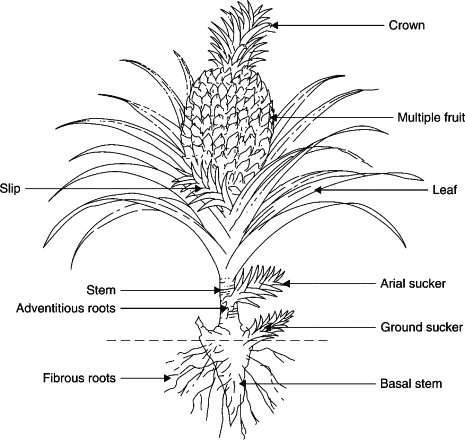
\includegraphics[width=6cm]{fig/pineappleStructure.png}

\scriptsize Source: \cite{hassan2011pineapple}
\end{figure}


The main parts of a pineapple plant are the crown, the fruit, the slips, a short and thick stem, two suckers, and a rosette of long (0.50–1.8 m), narrow, fibrous leaves. The structure of the pineapple is depicted in figure \ref{pineappleStructure}. Pineapple leaves (PAL), the biggest part of the plant, has potential to be used as a by-product for the production of many materials, or the generation of energy. Today, the PAL are not used in any valorisation process due to technological barriers and unawareness by farmers and local communities of its commercial uses \citep{jawaid2020pineapple, yusof2015novel}. 

According to a study carried out by \cite{chen2020production}, 250 tonnes of fresh pineapple plant waste are produced per hectare. The process used in their experiment demonstrated a generation of 23.3 tons of dry fibrous fibre after drying and gasification of the pulp. Considering that pineapple plantations in CR covered 40,000 harvested hectares in 2019 and that the pineapple waste is generated every two years (after the second harvest), dry fibre amounts to roughly 466,000 tonnes every year in CR. That is, for each tonne of fresh fruit produced, approximately 150 kg of dry fibre are generated. This is a relevant amount of stubble that is not only being discarded, it is also causing productivity losses to the farmers and environmental externalities to the nearby communities.

The removal and valorisation of pineapple residues after harvesting can have long-term environmental and socioeconomic advantages if value-added products can be economically produced from the pineapple residues. Pineapples leaves have commercial application potential which can add value to pineapple cultivation, facilitate extra income for entrepreneurs and farmers, and lead to agricultural diversification. 

\end{comment}

\section{Extraction from the field}

1. Extraction from the field is a big part of the puzzle to valorise the PAL. It is also a hard puzzle to solve: machinery, slope of the fields, technology that is inexistent for these conditions. 

2. Tell what has been tried (there are some things documented, other ideas are from field observation and interviews). 

3. Explain why these inventions fail from a technical point of view, and what is thought to be the solution.

4. Explain how the extraction from the field can be performed practically. Machine/workers extracting, shredding in the field itself or transporting the whole plants.

5. I gather information on costs of machinery and productivity levels (expected extraction rate, fuel/energy consumption, etc) add display on table. Again, from literature and interviews, some would be estimates.

6. Explain the (dis)advantages of using different methods and what they entail for the rest of the production of PAL-based goods (if shredding in the field then fibre is no option, for example).

\section{Potential uses of valorising pineapple stubble}

1. An in-detail description of the valorisation options being studied/implemented in CR. Stage of development and application. 

2. Costs (if available or if possible to estimate). Prices (if available or if possible to estimate). Their demand of PAL and their output estimates per tonne of PAL. 

3. A table is convenient here. It would be a good summary of the options.

\section{Demand for the potential PAL-based products}

1. Explain what is the (potential) demand of PAL-based products. I expect to give estimates based on available data online.

2. For example, for biogas, explain what can be done with it (selling to the ICE is not profitable). For fibre, there's no industry in the country. For silage, the ranchers think it makes no sense to buy it, etc.

\section{Local context and regulations applicable to PAL valorisation in CR}

1. Here I explain how regulations can affect the valorisation options.

2. Examples of what would go in this section: You cannot sell electricity privately. The bioethanol is regulated by Recope. If you want to make biobased materials to replace plastic, these must meet certain criteria, etc.


\newpage\cleardoublepage
\chapter{Harvesting The Fruits of Uncertainty}
\label{chapter_3lab}

The first study of a pineapple leaf valorisation process published in Costa Rica is a dissertation by \cite{quesada2003utilizacion}, who analyses the use of PAL as a polyester resin reinforcement. Since then, numerous studies in the natural and social sciences related to PAL valorisation processes have been published in Costa Rica and elsewhere. Yet, after two decades of the creative dissertation's publication, the valorisation of PAL has not taken off in Costa Rica. 

This chapter is devoted to explaining the complexity of the system in which the valorisation of PAL in Costa Rica occurs. To advance in the implementation of valorisation, we first need to understand why valorisation has not taken place and what are the barriers preventing it. Only then we can theorise what can be done to bring down those barriers and which stakeholders can lead the way in the circular economy.

\section{Theories on Circular (Bio)Economy}
\label{theoryframe}

 Due to the novelty of PAL valorisation and the complexity of the system in which it takes place, it is appropriate to define the concepts and discuss the theories that relate to the subject under study. There are several interlinked concepts we find relevant to discuss: the circular economy, the bioeconomy, the intersection of the last two, and the circular economy in the agricultural sector. Additionally, we discuss theories that serve to delineate the scope of our study.  Drawing from \cite{gottinger2020studying}, we describe how the Technological Innovation Systems (TIS) and similar frameworks can be used to identify the factors influencing transitions to a circular (bio)economy. The analytical framework designed by \cite{blomsma2022making} based on action recipes helps us to understand how circular-oriented innovation (COI) processes unfold.

\paragraph{Circular Bio(Economy)} \mbox{}\\
 The definition of circular economy varies in the literature and \cite{kalmykova2018circular} present the commonalities found among them. The first commonality is the maximisation of the value of the resources in use, also called stock optimisation. Eco-efficiency is also commonly mentioned when defining CE, sometimes as a consequence of it, other times as a purpose, and in some cases as a synonym. Yet, the authors remind us that eco-efficiency can also be achieved in a linear economy and that CE should rather aim to be eco-effective. The latter focuses not only on minimising the cradle-to-grave flow of materials but also on generating cyclical, cradle-to-cradle processes. Another concept often mentioned is waste prevention, which is frequently presented as the main purpose of CE. Finally, the four Rs (Reduce, Reuse, Recycle and Recover), the mechanism for achieving CE, is another shared feature among the CE definitions. 

There are also differences between the definitions that relate to the tightness of the loop within a value chain, that is, how closely the phases should be, and to the scope, which refers to the included resources: all physical resources or only certain sectors, products, materials, and substances. Because of these differences and because the shared features are not present in all definitions, \citeauthor{kalmykova2018circular} conclude that there is no established common ground for the variety of existing CE conceptualisations. Essentially, CE is a combination of several sustainability concepts and draws on other sustainability fields to construct its strategies. 

The concept of bioeconomy is commonly used alongside that of the circular economy. Their relationship and their differences as noted by \cite{carus2018circular} serve useful in our framework. Bioecomy involves the production of renewable biological resources and their conversion into value-added products, such as food, feed, biobased products, and bioenergy. The objectives of the bioeconomy are the introduction of healthy, safe and nutritious food and animal feed; the provision of bioenergy and biofuels to replace fossil energy; the development of new, more efficient, and sustainable agricultural and marine practices, the mitigation of climate change through the substitution of petrochemicals by materials with lower GHG emissions, and fossil fuels by biofuels; and the emergence of new business opportunities, investment and employment to rural, coastal and marine areas, fostering regional development and supporting small and medium enterprises.

Both the bioeconomy and the circular economy aim to avoid the use of additional fossil fuels and to a more resource-efficient system. As \cite{carus2018circular} clarify, the circular economy and the bioeconomy are two different yet complementary approaches to promoting sustainability. The circular economy focuses on improving resource efficiency and reducing the use of fossil fuels by incorporating recycled materials into processes. Bioeconomy aims to replace fossil fuels with biomass derived from agriculture, forestry, and marine environments. The intersection between the two concepts, the circular bioeconomy, can be interpreted in many ways. \cite{tan2021circular} mention that the relationship between CE and bioeconomy is complex and explain that the circular bioeconomy is more than the intersection of both concepts, their combination results in a more sustainable framework. Perhaps more useful is to look at their limitations to understand their differences. CE focuses on economic and environmental benefits while ignoring the social dimension. Moreover, efficiency gains can be confronted with rebound effects in the form of increased production and consumption. As for the bioeconomy, this cannot bring the perceived environmental benefits only by substituting fossil-based resources with bio-based ones.

It is important to note that both the CE and the bioeconomy are focused on resources, i.e., they deal with the cycle of materials, but they ignore the relationship between this cycle and broader ecological processes and ecosystem services such as water, nutrient cycles, quality of the energy source, and protection of biodiversity and ecosystems. In this sense, we find relevant the study by \cite{velasco2021circular} on CE in the agricultural sector. As the authors define it, apart from the components of the CE defined above, the CE in agriculture should also guarantee the regeneration of biodiversity in agroecosystems and the surrounding ecosystems. Additionally, they identify the main differentiating characteristics that must be considered in a CE framework for the agricultural sector. These are the perishable nature of products, the close link with natural ecosystems, and the strong seasonality of production. 


\paragraph{Transition towards a Circular Bioeconomy} \mbox{}\\
In their literature review, \cite{gottinger2020studying} provide an analysis of the different theoretical frameworks used to study the transition towards circular bioeconomy (CB). They conclude that the Technological Innovation Systems (TIS) framework has empirically served as most useful to identify influential factors to transition. \cite{markard2008technological} define TIS as \textit{a set of networks of actors and institutions that jointly interact in a specific technological field and contribute to the generation, diffusion and utilisation of variants of a new technology and/or a new product}. Actors can be individuals, companies, or governmental and non-governmental organisations. Institutions are the regulations and norms that influence the actions, decisions, and processes of actors. The networks can be learning networks that create knowledge bridges, or they can be policy networks linking actors with the same beliefs and agenda. In TIS, barriers are called blocking mechanisms, which hinder technology diffusion and industry development. The concept of system weaknesses is also commonly used in the framework and is usually the focus of the analysis when considering policy interventions \citep{giurca2017forest}.

Most studies assessing the CB transition analyse the strengths and weaknesses of innovation systems, the impact of certain events on the transition, and the facilitators of the transition. Less often, studies analyse the stakeholders, their roles and expectation towards the transition, and the interaction among them. A group of studies also focus on the changes that occur within existing sectors and their role in the transition. Finally, policies and their effects were studied in specific countries or by comparing policies cross-nationally.

\citeauthor{gottinger2020studying} identify six categories commonly found in the literature of barriers to transition toward CB.  
First, \textit{Policy and Regulation} is related to barriers associated with existing or missing policies and regulation implementation problems.
The category of \textit{Technology and Materials} encompasses the technical challenges associated with the application of technology and the creation of products, as well as the availability of input materials and physical infrastructure. 
\textit{Market and Investment} conditions refer to obstacles related to market demand and creation and the mobilisation and availability of financial resources. \textit{Social Acceptance} includes barriers associated with public awareness, interest and participation, as well as opposition from the public. \textit{Knowledge and Networks} encompass barriers linked to generating and applying knowledge, as well as the existence and development of efficient networks. Finally, \textit{Sectoral Routines and Structures} contains barriers associated with willingness and restrictiveness to change, such as risk-averse attitudes. From the analysed frameworks, TIS discovers a more extensive range of subcategories.

\paragraph{Circular-Oriented Innovation (COI)} \mbox{}\\
A big challenge in achieving a circular bioeconomy is to find ways to maximise the use of resources and, at the same time, convert them into value-added products. Thus, innovation plays a crucial role in driving the transition to a circular economy, as it enables the development of new, more sustainable, eco-efficient, and hopefully eco-effective, business models and processes. In this sense, \cite{blomsma2022making} explain how the processes of circular-oriented innovation (COI) occur. They draw from different organisation science frameworks to examine what strategies COI practitioners find relevant and how they employ CE action recipes, i.e., relationships between concepts and actions that help to clarify how ambiguity is addressed to enable action. They structure their framework by asking the following questions: 1) What is the motivation to engage in COI? (Which residues are present and where are they?), 2) How are circular strategies visualised to address the perceived issues? (Which circular strategies are applied and where?), 3) Who should act to implement them? (Which actors?).

Surprising or not, \citeauthor{blomsma2022making} find that the motivation to engage in COI consists of a complex mix of factors. CE solutions aim to address multiple problems, often in the form of structural wastes where there is lack of closing loops and preventative strategies. Additionally, CE practitioners identify benefits, such as larger profit margins or uncoupling from raw materials that will be scarce in the future. Answering the second question, they mention that circular strategies require linking knowledge and stakeholders in a manner not previously employed in the linear economy. Because circular strategies in complex real-life cases are not usually employed individually and instead interact with each other, an understanding of these synergies is required. This relates to the fact that CE is an umbrella term that, as mentioned before and explained by \cite{kalmykova2018circular}, draws from different sustainability strategies. Finally, the answer to which action is needed to implement CE solutions is focused on value network dependencies. The difficulties that COI practitioners face as CE strategies progress are related to the dependence on other actors within the system. Additionally, \cite{blomsma2022making} remark on the importance of deciding when stakeholders should be involved in innovation processes. Early engagements can hinder certain CE solutions, and sometimes it is best to wait until a solution is better developed to seek collaborations. Finally, by identifying the CE action recipes, some of the barriers initially defined as important by practitioners can be discarded later in favour of fewer but more central barriers. By focusing on a subset of barriers, innovators can take action more easily, which also allows them to take further steps more easily in the future. Nevertheless, this idea raises the question of when a circular solution can be considered to be sufficiently developed. In this sense, the authors recommend taking a sufficiently long time horizon to understand circular phenomena in business. 

As mentioned above, value network dependencies play a relevant role in COI implementation. Therefore, we find it useful to look into how collaboration takes place in COI more deeply. \cite{brown2019companies} provide an insight into the motives, barriers and drivers that stimulate or hamper collaborative innovation within the context of CE. They divide the identified motives into intrinsic (realised for their own sake), and extrinsic (realised for external recognition). Both can originate from the personal and organisational levels. For example, responsibility for sustainability can have intrinsic and extrinsic motives, and such motives trigger collaboration with other actors if both parties feel alignment between their motivations. Moreover, the recognition of interdependence also stimulates collaboration. The complexity of CE strategies and the dispersion of knowledge among stakeholders drives this interdependence. 

Another motive driving collaboration is the necessity to find suitable experimental arrangements. These arrangements break down complex systems into manageable projects. Then, experimentation helps in creating knowledge, and in engaging stakeholders to develop evidence that helps overcome barriers to adopting CE strategies. Testing at scale is important to identify unintended or unexpected impacts in the system, and collaboration is necessary to share the potential risks and costs. The last motive that stimulates collaboration identified by \citeauthor{brown2019companies} is the need to implement the business model. This motive is not as developed because technical innovation is usually more advanced than market/business model innovation. Collaboration is needed to develop all the operations required for CE strategies, but there is less collaboration in this area due to competition. In this sense, a clear barrier to collaboration in the context of COI is the contradiction of companies wanting to share but also protect knowledge. Moreover, sharing economic rewards becomes more difficult as companies prioritise individual returns over the shared benefits drawn from the project. This creates a cultural barrier that can hinder the progress of collaborative innovation efforts beyond the experimental phase. 

If the culture in the organisations involved in COI is not aligned, the shared CE objectives will not develop. The challenge is to increase internal motivation and change culture before even achieving evidence of CE. As concluded by the \citeauthor{brown2019companies}, COI is confronted with the challenge of transitioning from exploring new market opportunities and closed-loop experiments to initiating societal transformations through larger-scale collaborations. This necessitates overcoming barriers related to organisational mindsets and collaborative knowledge sharing. The latter requirement is a shared concept among CE frameworks. For example, \cite{antikainen2016framework} highlight the importance of the interaction between stakeholders when building CE business models. Their study corroborates the idea that CE business models are not isolated but rather integrated into a system of business models that together close a material loop. COI, in this sense, requires the collaboration and communication of many parties.

Inventions do not necessarily bring innovation. When we analyse the valorisation of PAL, we can think of it merely as the invention of a new product and the recycling of agricultural residues, or we can see it as part of an innovation process driven by many stakeholders for a sufficiently long period to transition to a more circular economy. Whether PAL valorisation remains an invention or progresses to become an innovation depends on the capacity of the industry and stakeholders to overcome the barriers preventing its implementation and to exploit its linkages to the circular bioeconomy revolution.

\begin{comment}
....................

Technology acceptance model: This theory can be used to understand the factors that influence the adoption and usage of new technology. In the context of transitioning to circular management of pineapple stubble, the technology acceptance model can be used to identify the technological and cultural barriers that prevent stakeholders from adopting and utilising circular practices.

Resource dependence theory: This theory can be used to explain how organisations are dependent on their environment for resources and how they manage their dependencies. In the context of pineapple stubble, resource dependence theory can be used to understand the interdependencies of actors in the industry and how they may affect the adoption of circular practices.

Institutional theory: This theory can be used to explain how institutional norms and values shape the behaviour of actors in an industry. In the case of pineapple stubble, institutional theory can be used to understand how cultural beliefs and practices, as well as regulatory frameworks, may inhibit the adoption of circular practices.

Socio-technical systems theory: This theory can be used to understand the interactions between social and technical components of a system and how they influence each other. In the context of pineapple stubble, socio-technical systems theory can be used to understand how social, cultural, and technical factors interact to prevent the adoption of circular practices.

Prospect theory: This theory explains how people make decisions under risk and uncertainty. In the context of pineapple stubble, prospect theory can be used to understand how risk-taking aversion among companies may inhibit the adoption of circular management practices.

Real options theory: This theory can be used to understand how firms make investment decisions under uncertainty. In the context of pineapple stubble, real options theory can be used to understand how companies may perceive the uncertainty of the benefits of adopting circular management practices as a barrier to their adoption.

Innovation adoption model: This theory can be used to understand the factors that influence the adoption of innovations by organisations. In the context of pineapple stubble, the innovation adoption model can be used to identify the factors that influence the adoption of circular management practices, including the perceived risks and uncertainties associated with the transition.

\end{comment}

\section{Methodology}

\subsection{Fuzzy Cognitive Maps for Knowledge Elicitation and Analysis}

A lot of knowledge is created in the process of innovation. Many times, this knowledge can be dispersed, or fuzzy. The fuzzier the knowledge representation, the easier the knowledge acquisition, but also the harder the knowledge processing. In such cases, Fuzzy Cognitive Mapping (FCM) serves as a great tool for eliciting this fuzzy knowledge because it allows fuzzy degrees of causality between causal concepts \citep{kosko1986fuzzy}. 

FCM is a technique that builds quasi-quantitative models from the knowledge of interconnected variables in a system. It was first introduced by \cite{kosko1986fuzzy}, who presented FCM as a tool to model complex systems and decision-making. Fuzzy Cognitive Maps are composed of a set of nodes that represent the variables or concepts of the system and a set of links between them that represent the relationships between the variables. Each link is associated with a weight that represents the strength of the relationship between the variables. These weights can be positive or negative and, thus, variables can ``decrease'' or ``increase''. A simple example of an FCM with three concepts and four connections is presented in \cref{example_fcm}. The connections between the variables in the system represent causal influence. Exploring how these causal influences propagate through the system when it is subject to change or intervention is the main objective of FCM \citep{barbrook2022systems}.

\begin{figure}[H]
\caption{Example of a Fuzzy Cognitive Map}  
\label{example_fcm}
\centering
\includesvg[inkscapelatex=false,width=8cm]{fig/fuzzyExample.svg}
\end{figure}

There are two main approaches to using FCM. The ``causal" approach implies that the strength of links between concepts represents how certain the experts are that a factor causes, or suppresses, another. The ``dynamical" approach models the propagation of effects of one concept on another, resulting in a representation of the relative magnitude of changes in concept values. This approach allows us to understand which concepts are the most important or the most influenced in a system. In our study, we use the dynamical approach because it reflects a widespread usage of FCM in a participatory manner and allows for a better interpretation of cognitive maps.

The FCM modelling technique allows for more nuanced modelling of relationships that better reflect the uncertainty and ambiguity that are often present in real-world systems. As \cite{ozesmi2004ecological} explain, FCM can involve local people who typically possess a comprehensive understanding of the ecosystem and whose participation and input can be crucial for informed decision-making and for gaining acceptance from the public for the proposed solutions. Furthermore, ``wicked" environmental problems that involve many stakeholders and which have no easy solutions can benefit from a model that brings together the knowledge of different experts from different disciplines and compares their perceptions. In this way, FCM can help to understand the advantages and disadvantages of possible decisions. Finally, it is important to highlight the benefits of the interaction between the researcher and the stakeholders throughout the analysis. As a participatory approach, FCM allows for recursive feedback, which helps to model an accurate representation of reality. Moreover, this approach provides the stakeholders with the opportunity to reflect on the problem at hand; the process of building a Fuzzy Cognitive Map is as important as its results. 

The use of FCM in the field of environmental studies is extensive, covering climate change \citep{kontogianni2012you, singh2014livelihood, reckien2014weather}, deforestation \citep{kok2009potential}, fire ecology \citep{devisscher2016anticipating, eriksson2022using}, pollution \citep{anezakis2016fuzzy, salberg2022assessing, ozesmi2003participatory}, renewable energy \citep{jetter2011building, alipour2019characteristics, kyriakarakos2014fuzzy}, urban ecology \citep{assunccao2020rethinking, olazabal2016use}, water use \citep{giordano2005fuzzy, kafetzis2010using}, and waste management \citep{falcone2020use, morone2021using, kokkinos2018fuzzy, konti2018exploring}. 

There are many ways of developing and applying Fuzzy Cognitive Maps, but the structure is regularly the same. We find that the six steps proposed by \cite{edwards2021building} and illustrated in \cref{stepsFCM} are suitable for our case. The authors implement an episodic and asynchronous method with the participation of stakeholders on two occasions. The process starts by determining the scope and objective of the study, which results in the design of an interview outline. The second step is the selection of stakeholders. Then, stakeholders are consulted to generate knowledge by means of in-depth individual interviews. The fourth step consists of the qualitative aggregation of concepts, in which the interviews' output is analysed and harmonised. In the fifth step, stakeholders participate for the second time to weigh the connections identified in the previous step, resulting in individual fuzzy cognitive maps. The last step involves combining the responses to generate the aggregated FCM and further analyse it. In the following sections, the implantation of these steps for our case is explained in detail.

\begin{table}[H]
\centering
\resizebox{\textwidth}{!}{
\begin{threeparttable}
\caption{Fuzzy Cognitive Map Building Steps and Products}
\label{stepsFCM}
\begin{tabular}{lll} \hline \hline 
       & Process                           & Product                                            \\ \cline{2-3} 
Step 1 & Definition of objective and scope & Interview Questions                                \\
Step 2 & Stakeholder selection             & List of Participating Stakeholders                 \\
Step 3 & Knowledge generation              & Original concepts and connections                  \\
Step 4 & Qualitative aggregation           & Generalised labels for concepts, added connections \\
Step 5 & Weighting connections             & Individual FCMs                \\
Step 6 & Quantitative aggregation          & Aggregated FCM   \\ \hline   \hline     
\end{tabular}

\begin{tablenotes}
      \small \item Adapted from \cite{edwards2021building}
\end{tablenotes}
\end{threeparttable}%
}
\end{table}


\subsection{Definition of objective and scope}

We begin by defining the objective and scope of the FCM study which, as explained by \cite{edwards2021building}, guide both stakeholder identification and the questions posed to elicit knowledge about the system. In this chapter, we try to achieve the first objective defined in the Introduction: to understand why the valorisation of PAL has not taken off in Costa Rica. Thus, the scope, which refers to the study area we try to describe, is at the national level. The main question is \textit{What are the barriers preventing the valorisation of PAL in Costa Rica?} Thus, PAL valorisation is the first and central concept of the FCM. Finally, we define the interview questions to be asked to the stakeholders in the third step. It was decided to formulate open-ended questions to allow the interviewees to elaborate on their answers; this is often the domain of qualitative research \citep{barbrook2022systems}. The interview template is shown in \cref{interviewOutline}.
  
\subsection{Stakeholder selection}

When implementing FCM, it is important to represent all the people who impact or are affected by the system under study. A good way to determine whether the population to be represented has been sampled sufficiently is to check the number of new concepts added by each new participant. \cite{ozesmi2004ecological} examined accumulation curves of the total number of variables versus the number of interviews, as well as the number of new variables added per interview, using Monte Carlo techniques. Their results, depicted in \cref{accumFCM}, show that as the number of interviews increases, the number of new variables decreases and that the total number of variables increases at a decreasing rate. This behaviour is normal if we consider that most stakeholders in the system share the same vocabulary about the subject of enquiry. A similar result can be found in \cite{morone2021using}, whose research demonstrates how the generation of new variables decreases rapidly. However, \cite{ozesmi2004ecological} note that we can expect one or two new variables to be mentioned for each new interview. 

\begin{figure}[ht]
\caption{Accumulation curves of concepts versus interviews} \label{accumFCM}
\begin{subfigure}[b]{0.45\textwidth}
  \centering
  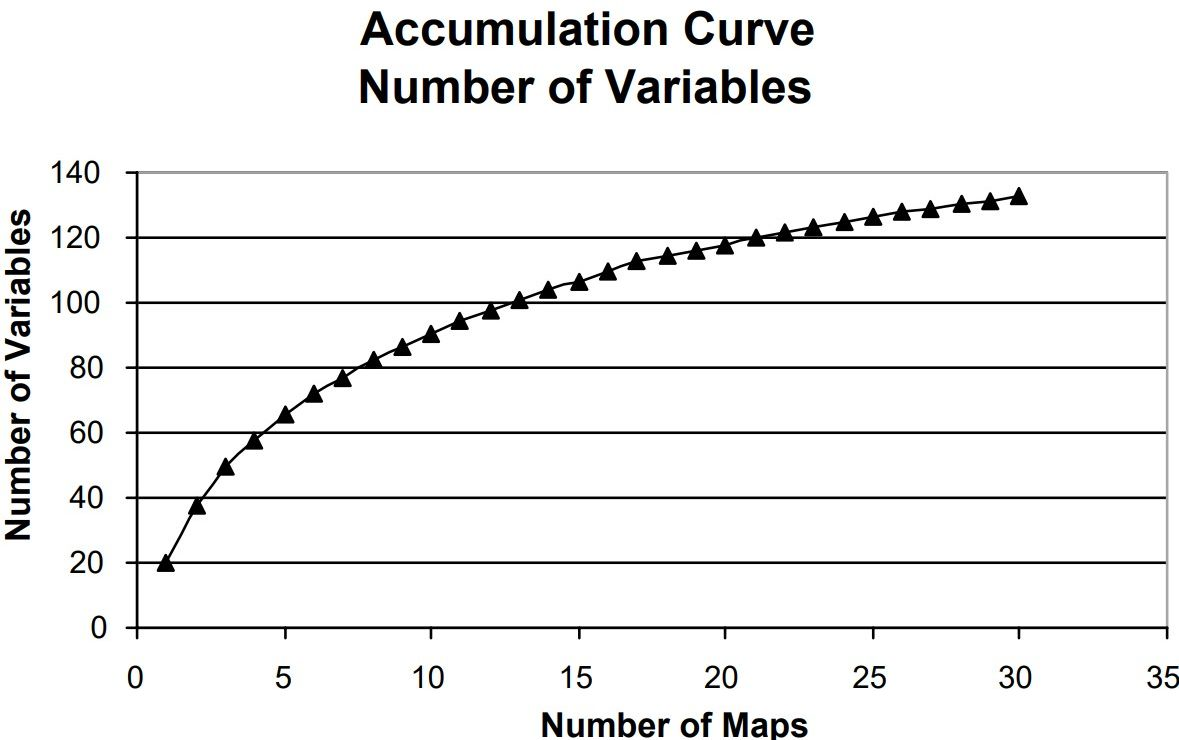
\includegraphics[width=\textwidth]{fig/numVars.jpg}
\caption{Number of variables vs. number of maps} 
  \label{accumFCM:sub1}
\end{subfigure}%
  \hfill
\begin{subfigure}[b]{0.45\textwidth}
  \centering
  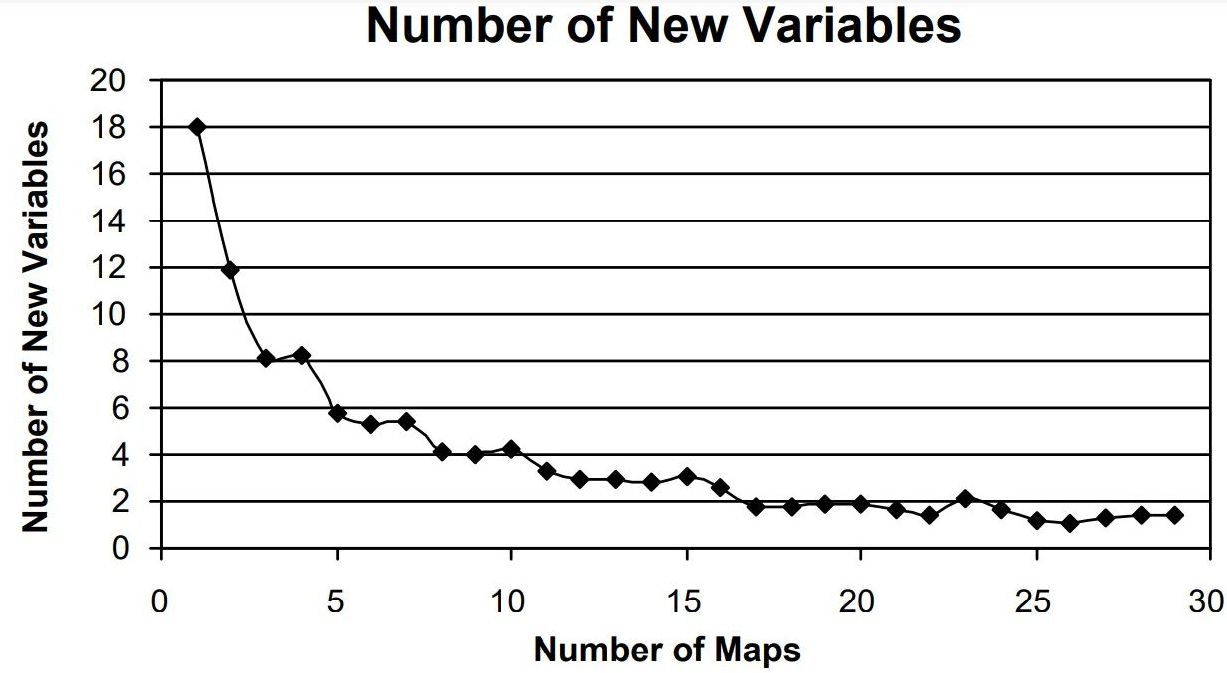
\includegraphics[width=\textwidth]{fig/newVars.jpg}
\caption{Number of new variables added per map}    
  \label{accumFCM:sub2}
\end{subfigure}
%\captionsetup{justification   = raggedright, singlelinecheck = false}
\caption*{\textit{Source:} \cite{ozesmi2004ecological}}
\end{figure}

It is useful to think of categories when selecting stakeholders in the system, and then identify individuals who fit the categories. As such, in our case study, we defined three broad categories: research, government, and industry. Once contact was made with an individual within each category, more participants were identified by snowballing. 

\subsection{Knowledge generation}

\cite{edwards2021building} highlight how important it is that the researcher designs and executes stakeholder engagement during their participation in the knowledge elicitation process so that their perspective is represented in the final product of the FCM. At this stage, the researcher decides the balance of coproduction, i.e., how much stakeholder input and researcher input are used in the process. Semi-structured in-person interviews were held separately with each identified stakeholder. It is important to have a structured interview process that allows for the collection of detailed information, while also giving the interviewee the freedom to share the information they deem most important. In the interviews, the stakeholders were first introduced to the objective and scope of the study. Then, the predefined questions were asked and, depending on the interviewees' responses, additional questions were posed to clarify or augment the information provided. No concepts were provided to stakeholders, but it was ensured that the focus was kept on the valorisation of PAL. The interview sessions lasted between 40 and 120 minutes, were conducted between August and November 2022, and were recorded when the respondents gave their consent. 

\subsection{Qualitative aggregation}

The recording of the interviews was transcribed using Whisper, a general-purpose speech recognition model. The script used for the transcription can be found in the Supplementary Material. The transcription of the interviews along with the notes taken by the researcher was used to create a list of concepts mentioned by the participants. In cases in which the interviewees defined the same concept using different vocabulary, the definitions were grouped into one concept. As concepts were identified, connections were established as well. 

In \cref{process_fcm} we demonstrate how the following statement made by one of the stakeholders was converted into four concepts and three connections: ``[W]hat we are looking for with the recovery of stubble is ... converting something that today is waste into a value-added product. [A]n economic benefit, but also a social and environmental benefit. For example, if we avoid the fly problem, we already have an important environmental benefit." This is a straightforward example, as it includes the central subject of study, the valorisation of PAL, and its main consequences. 

In the figure, it can be observed how vocabulary harmonisation and concept grouping take place. In the first step, identified concepts and connections between them are extracted from the interviewee's statement. Then, the concepts \textit{Recovery of stubble} and \textit{Value-added products} are grouped into \textit{PAL valorisation}. \textit{Economic benefit} is translated into \textit{Increase profitability of the pineapple producers} because producers are assumed to be the ones that valorise PAL in most cases and because economic benefits is a broad concept that has a different definition for different stakeholders. For the second round of stakeholders' participation, it is important to use clear concepts that convey a similar definition to everyone. For this harmonisation process, analysis of commonly used terms used in the literature is also useful. The same explanation is valid for the translation of \textit{Environmental benefits} into \textit{Increase Community’s Health/Wellbeing}. 

In the third step, it can be observed how the concepts take their final shape. The impact previously denoted in words, increase and reduce, are now connections, represented by positive and negative signs. It is worth noting how this affects the relation between concepts: in step two, the community's health/well-being is enhanced because the stable fly is avoided as PAL valorisation takes place. In the FCM, this is represented by two negative effects, one from the valorisation of PAL to the propagation of the stable fly, and another from the latter to the community’s health/wellbeing. In this way, the effect of PAL valorisation on the community’s health/wellbeing is transmitted through a negative effect to and from the (presence of) stable fly. This simple example also shows how important it is to use concepts that behave like variables, i.e., that can be thought to increase or decrease. 

The concepts and connections shown in \cref{process_fcm} are only part of the FCM built for our case, and the displayed concepts can affect or be affected by many other concepts. The aggregation and harmonisation process exemplified here needs to be repeated by revisiting statements and checking the logic and internal consistency within the concepts and connections. As more statements from different stakeholders are analysed, concepts are renamed, and connections are added or deleted. Finally, we find a map that represents how stakeholders perceive the system dynamics and that can be understood with ease. 

\begin{figure}[H]
\caption[Example of interview statement processing]{Example statement processing to build FCM concepts and connections}
\label{process_fcm}
\centering
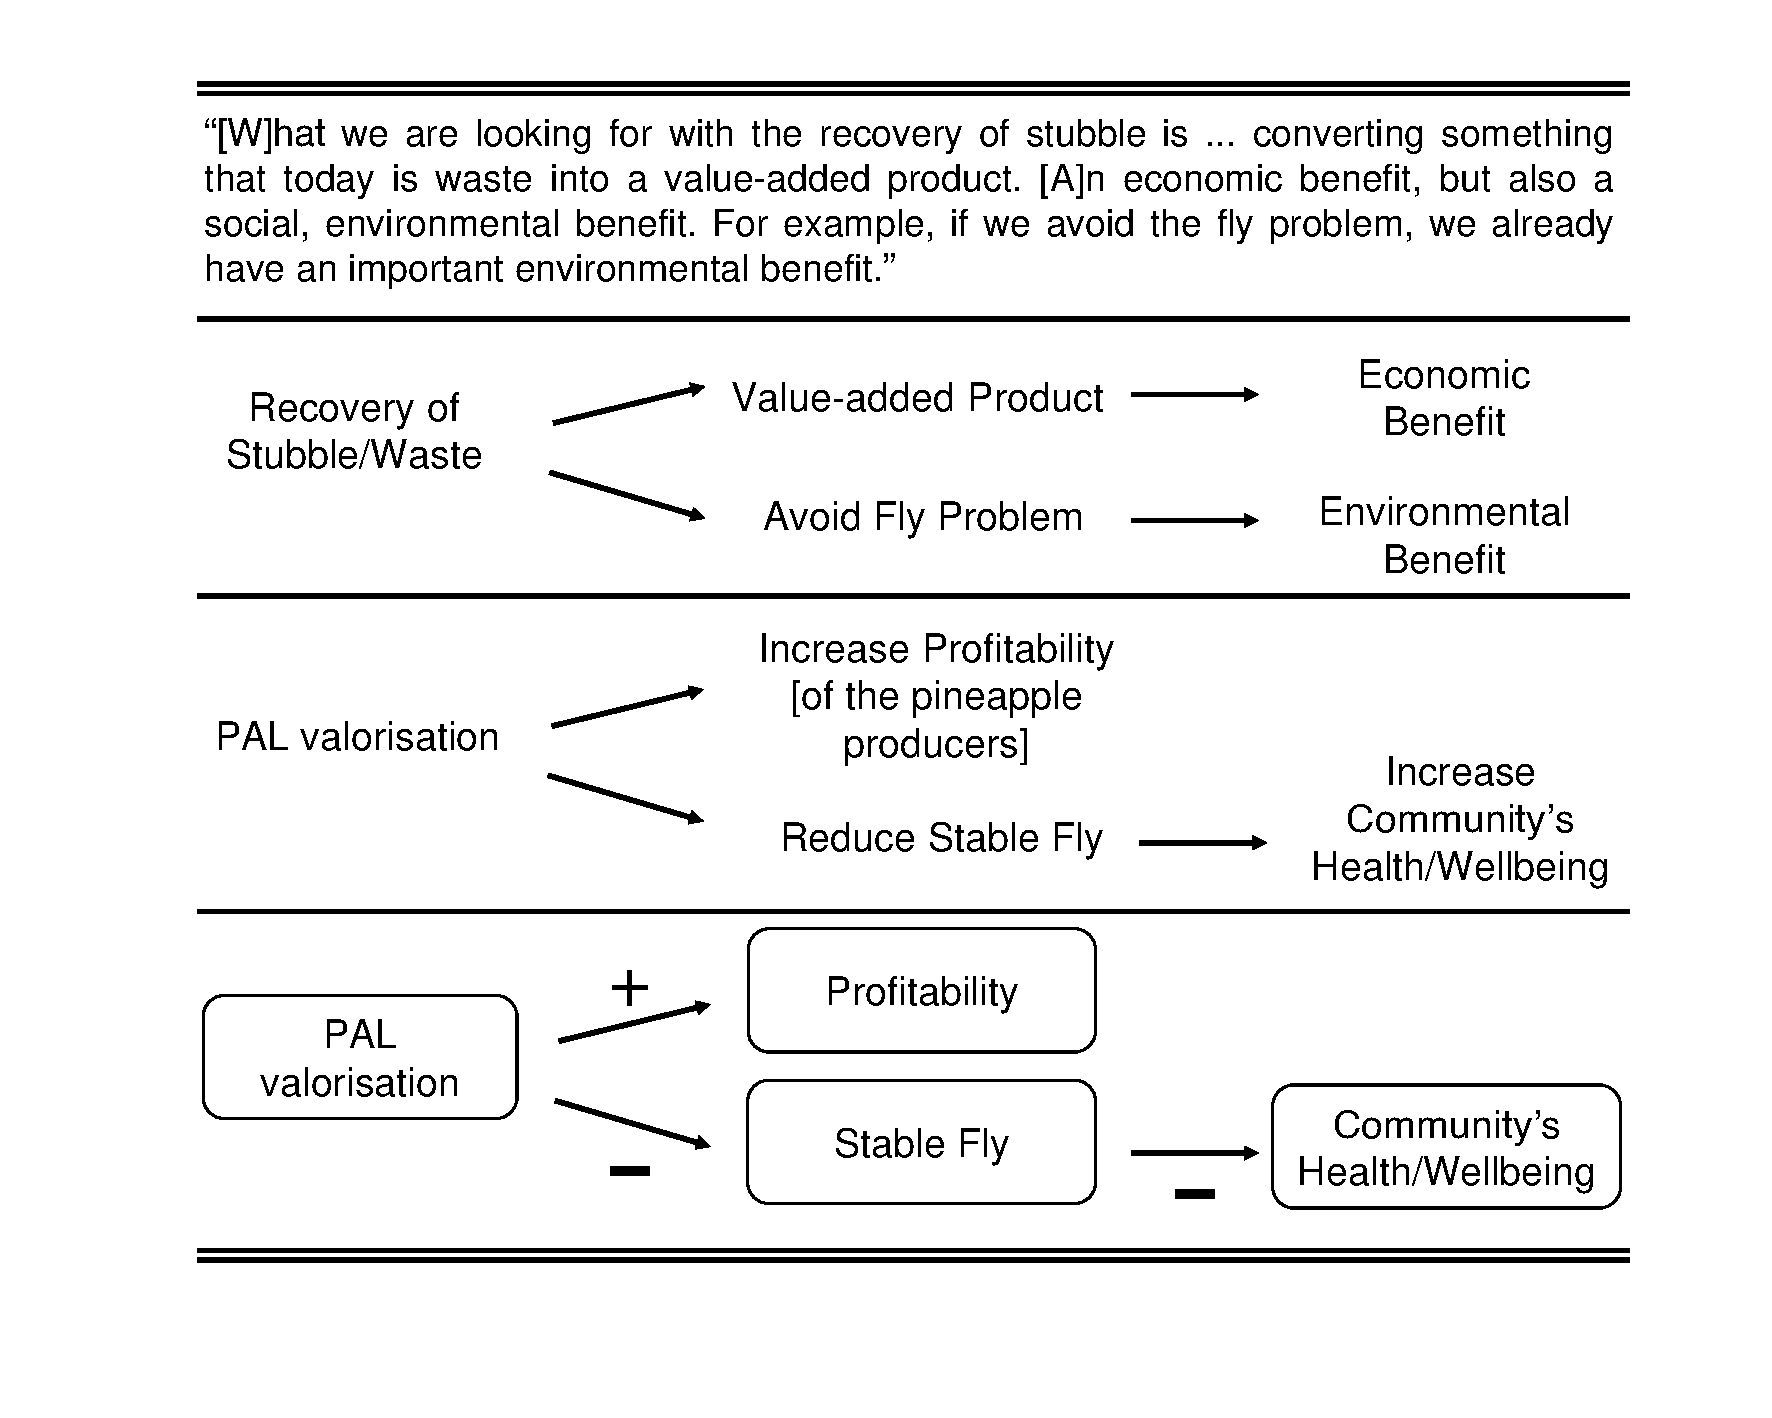
\includegraphics[width=\textwidth]{fig/processFCM.pdf}
\end{figure}


\subsection{Weighting connections}

After the concepts and connections are identified, the next step is to assign weights to the connections. For this purpose, a second round of participation from stakeholders is conducted using an online questionnaire. Qualtrics Online Survey Software was used to make the questionnaire form. For each connection, stakeholders were asked to assign a value to the strength they think exists between concepts. In the previous step, the sign of the connections was assigned based on what the majority of the statements from the interviews indicated. Thus, stakeholders were asked to indicate only the value of the connections. At the end of the questionnaire, respondents could comment on relationships or signs that they thought were incorrectly identified, or add new concepts and connections that they thought were missing. At this point, it is relevant to remind the reader that the FCM developed in this study is the so-called dynamical FCM, which means that the values represent the propagation of effects of one concept on another and not the measure of certainty that the stakeholder has of the connection. 

All the questions in the questionnaire followed the same structure ``If concept A increases, how much does concept B increase (decrease), on a scale from 1 to 5? (1 being increases (decreases) little and 5 being increases (decreases) a lot)". Initially, qualitative values --- Very High, High, Medium, Low, Very Low --- were used in the questionnaire, but it was soon realised that this, together with the sign of the connection, was confusing to respondents, and that a numerical scale, coupled with the terms increase and decrease to represent the sign of the connections, was simpler to interpret. The best way to formulate the questions is the one that works for the case and the target group, and examples of both qualitative and quantitative values can be found in the literature (e.g., see \cite{morone2021using} for the former and \cite{olazabal2016use} for the latter). A glossary containing all concepts and their definitions (see \cref{conceptsGlossary}) was provided with the questionnaire in case the respondents had doubts about what a concept term meant. At the end of the questionnaire, the output of the previous step, the visual map with all identified concepts and connections, was also provided to assist respondents in identifying missing concepts and connections. After four weeks of sending the questionnaire, the responses were collected to proceed with the final step in the process. 

\subsection{Quantitative aggregation}

For a comprehensive explanation of the quantitative aggregation process, we refer the reader to \cref{quantitativeAgg}

The data extracted from the questionnaire responses were transformed by converting the categorical ratings to an adjacency matrix. Sometimes, researchers use a scale to weigh the consistency of stakeholders' answers, giving more weight to experts who are believed to be more knowledgeable. In our case, we have assumed that all individual FCMs are equally valid and, thus, the same weight was applied to all maps when aggregating. 

With the aggregated matrix, we can perform a dynamic analysis of the FCM. As \cite{edwards2021building} mention, in a mathematical sense, the output of the analysis is static rather than dynamic, so they adopt the term ‘quasi-dynamic’ to indicate the dynamic character of the interpretation of the changes in the system. This quasi-dynamic analysis allows us to see where the system will go if things continue as they are, i.e., to determine the steady state of the system \citep{ozesmi2004ecological}. The steady-state value taken by each concept reflects its importance within the system according to stakeholders' knowledge and provides an idea of the evolution of the system in current circumstances \citep{lopolito2020combined}. 

To compute the steady state of the system, a vector of initial states of variables is first multiplied by the aggregated adjacency matrix of the FCM. Then, the resulting transformed vector is repeatedly multiplied by the adjacency matrix and transformed until the system converges to a steady state.  It is important to note that iterations are not related to time. This property allows an interpretation of the dynamics of the different factors relative to the other factors or relative to other descriptions of the system \citep{edwards2021building, diniz2015mapping}. In this sense, it is possible to evaluate different scenarios and outcomes by asking ``what-if" questions and simulating different conditions or policy choices. This can be used to compare what policy decisions or changes in the system would have the greatest effect on the variables of interest.

\section{Results and Discussion}

\subsection{Descriptive analysis}
\label{descriptiveFCM}

A total of 14 experts participated in the study. Three are classified as research related, one as government, and 10 as industry related. In the latter, we can find companies directly related to pineapple production and companies that are involved in PAL valorisation in some way. All stakeholders participated in the first round of participation, which consisted of one-to-one, in-person interviews. The online questionnaire, which took place in the second round of participation, was responded to by only half of the stakeholders. Four additional pineapple producers, two government agencies, and one company related to PAL valorisation were contacted to participate in the study, but no response was received. A list of stakeholders, their affiliation and role, and their participation in the participation rounds can be found in \cref{expertsList}.

\begin{table}[ht]
\centering
\resizebox{\textwidth}{!}{
\begin{threeparttable}
\caption{Profile, role and participation of stakeholders}
\label{expertsList}
\begin{tabular}{lcp{0.5\textwidth}cc} \hline \hline \\

Group & \begin{tabular}[c]{@{}c@{}}Respondent \\ Code\end{tabular}  & Role & \begin{tabular}[c]{@{}c@{}}Participation \\ in 1st round\end{tabular}  & \begin{tabular}[c]{@{}c@{}}Participation \\ in 2nd round\end{tabular}        \\ \hline
    Research & R1  & Works at university conducting research in  pineapple valorisation options      & Yes & Yes \\
                           & R2  &    Works at university conducting research in  pineapple valorisation options                                                                                              &               Yes        & Yes \\
                           & R3  & Agri-food research organisation involved in the design of an extraction machine                   &   Yes                    & No  \\ Government                 & G1  & Agency of the Ministry of Agriculture in charge of protecting agricultural resources from pests. &    Yes                   & No  \\
Industry & I1  & Small-scale farmer considering valorisation options                                              &           Yes            & Yes \\
                           & I2  & Large-scale farmer                                                                               &    Yes                   & No  \\
                           & I3  & Medium-scale farmer with various PAL valorisation projects                                       &    Yes                   & No  \\
                           & I4  & Large-scale farmer with a PAL valorisation business                                              &   Yes                    & Yes \\
                           & I5  & Large-scale farmer with a R\&D team researching valorisation options                             &    Yes                   & Yes \\
                           & I6  & Association of pineapple producers                                                               &      Yes                 & No  \\
                           & I7  & Company working on field extraction machine                                                      &     Yes                  & Yes \\
                           & I8  & Company marketing PAL as fodder                                                                  &      Yes                 & No  \\
                           & I9  & Company producing and marketing PALF                                                             &     Yes                  & No  \\
                           & I10 & State-owned enterprise that developed a PAL-based biogas plant                                                               &  Yes                     & No  \\ \cline{1-5} 
Number of participants  & & &  14 & 7 \\ \hline \hline
\end{tabular}
\end{threeparttable}%
}
\end{table}


The generation of knowledge by stakeholders in the interviews resulted in 32 concepts and 52 connections. The diagram representing the connections is presented in \cref{FCMdiagram}. A list with a description of the concepts, which was also shared with the stakeholders in the questionnaire, is shown in \cref{conceptsList}. A section to add comments was provided on the online questionnaire, and valuable feedback was given by three stakeholders. The stakeholders mentioned that some concepts were too broad and that narrowing the definition can make the connections clearer. They also mentioned a disagreement with the effect of the concept \textit{Profitability} on the concept \textit{Sustainability of the industry}; indeed, in the interviews, some stakeholders defined this relationship as positive, but the majority stated that it was negative. Finally, stakeholders emphasised the importance of transparency in the industry for the collection of data needed to conduct large-scale valorisation studies, and that the results of the small-scale studies that have been developed cannot be extrapolated. No further concepts or connections were added in this comment section. 

\newpage

\begin{landscape}
\begin{figure}[H]
\caption{FCM resulting from interviews}  
\label{FCMdiagram}
\centering
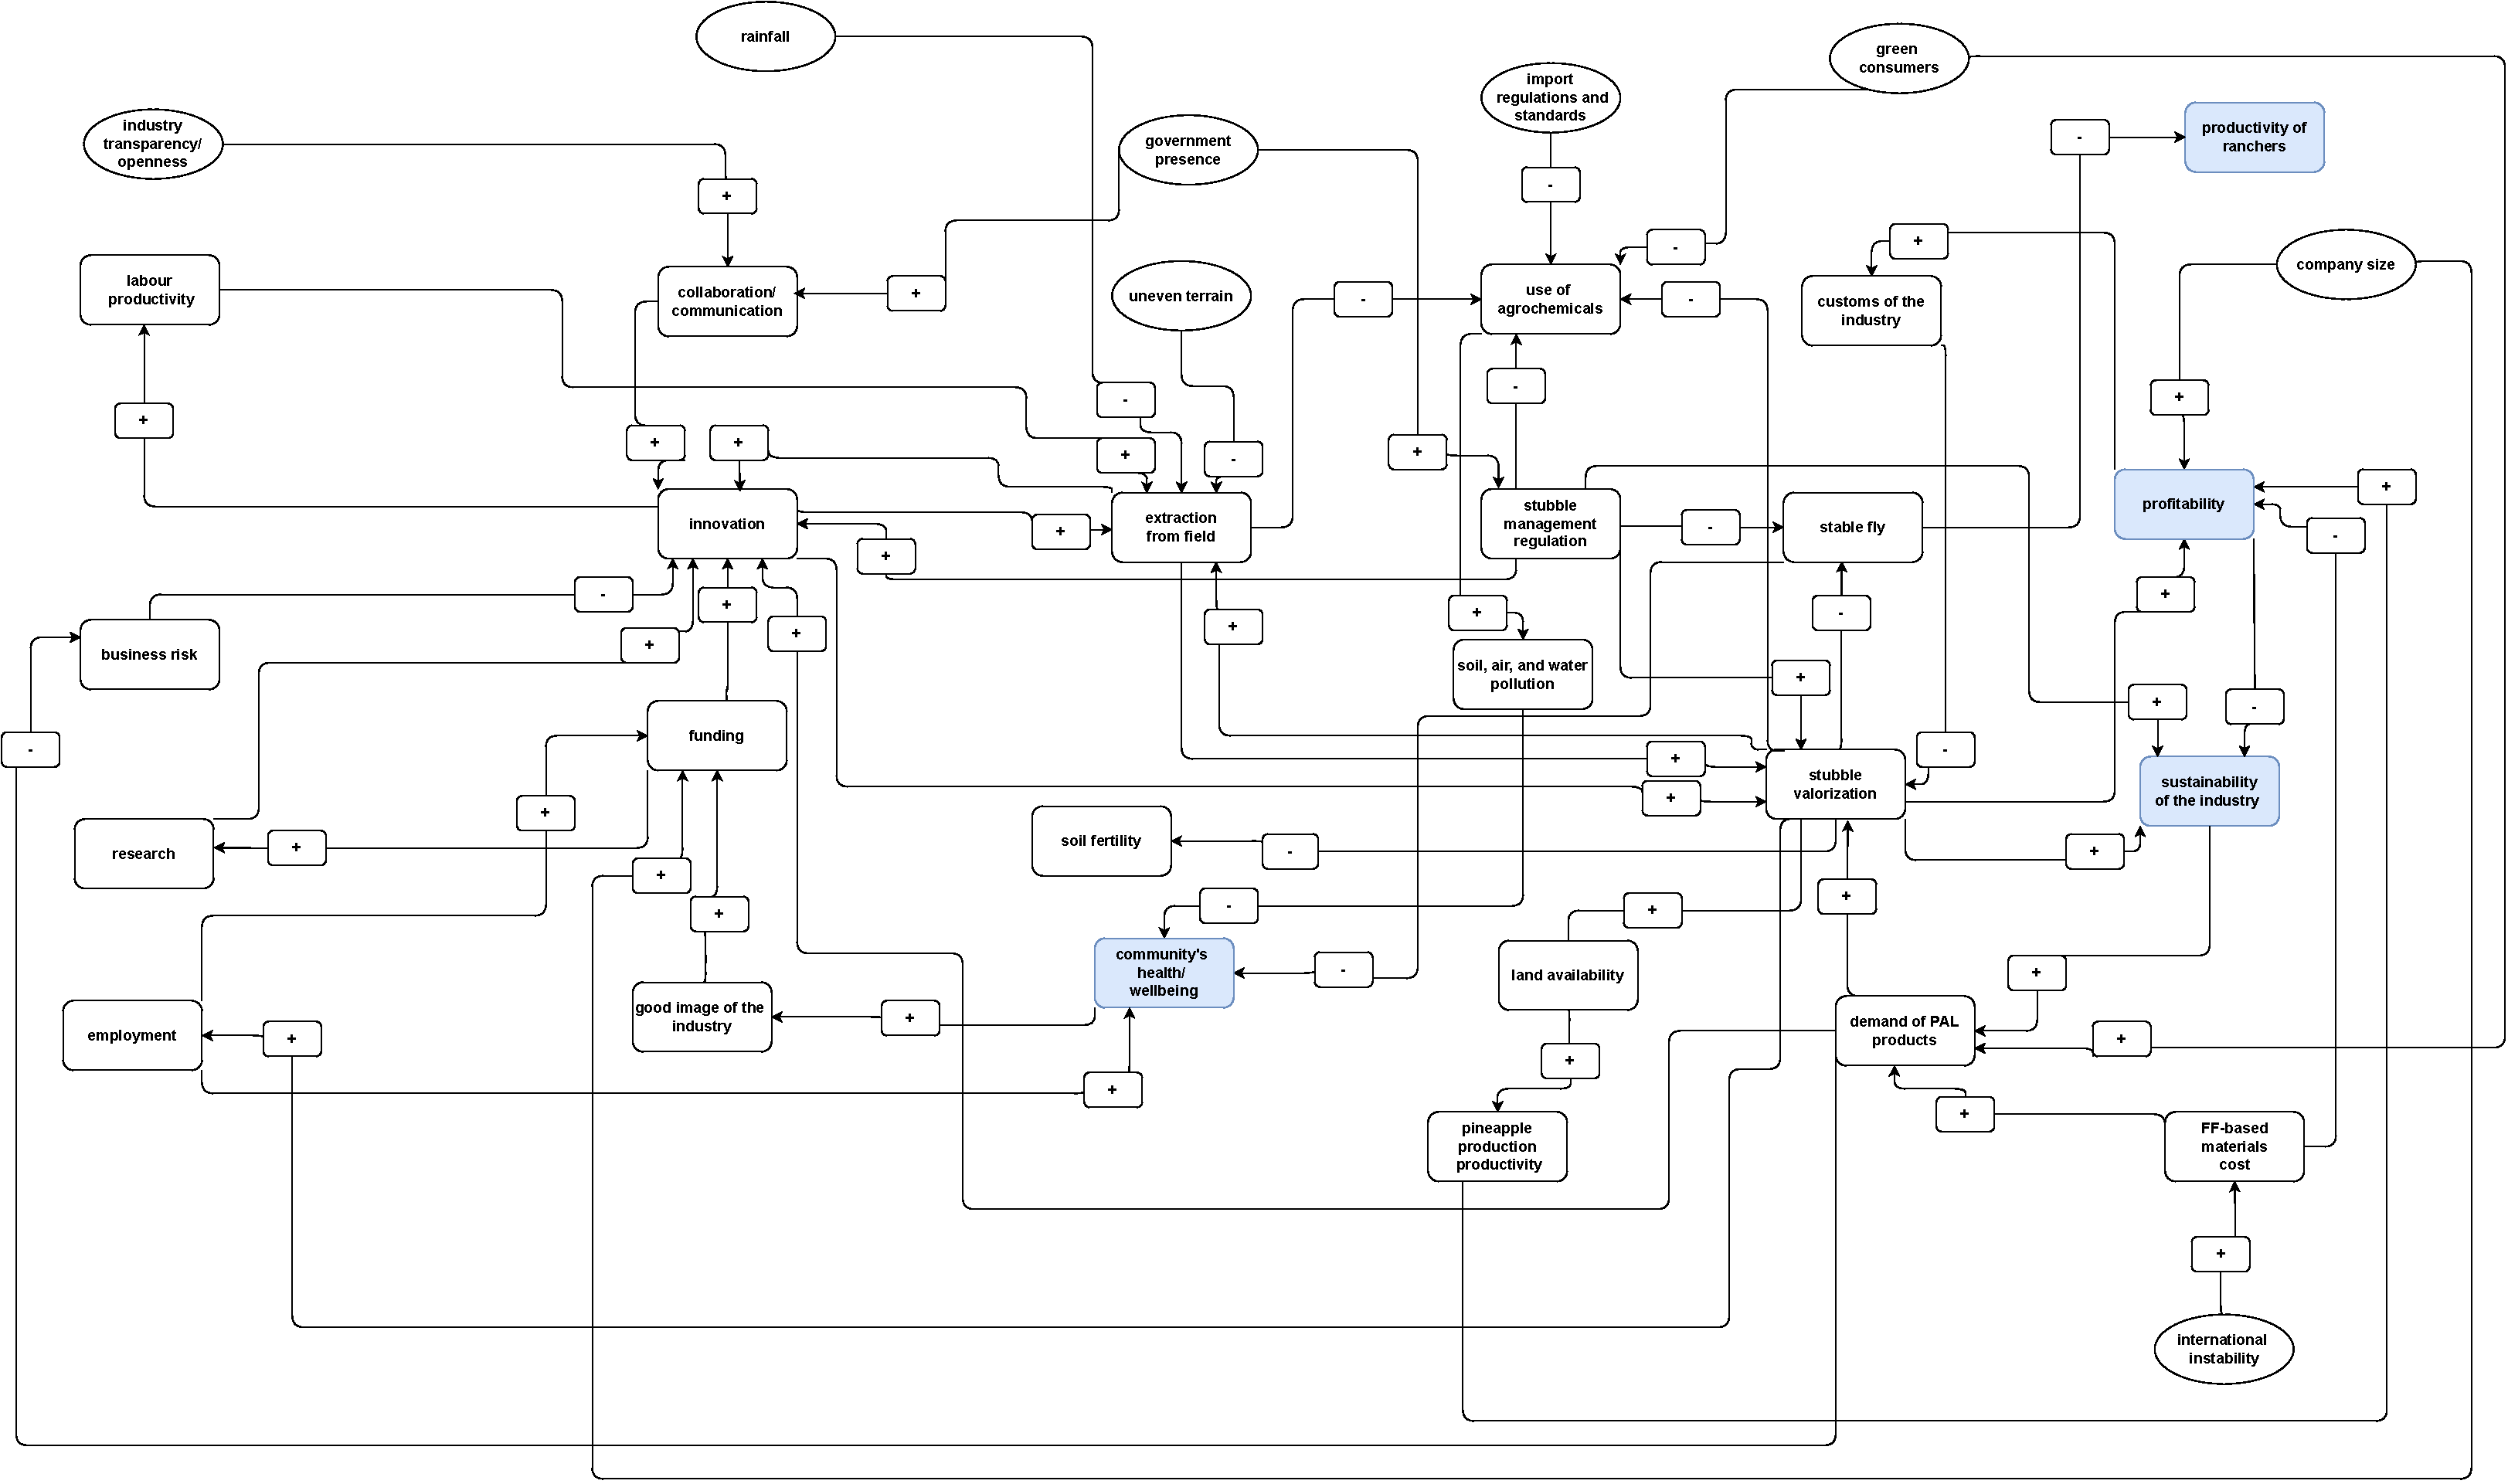
\includegraphics[width=23 cm]{fig/diagram.drawio.pdf}
\end{figure}
\end{landscape}

\clearpage

Most of the concepts were mentioned by more than one stakeholder. The most mentioned concepts, in addition to \textit{valorisation of PAL}, were \textit{Extraction from the field}, \textit{Innovation}, \textit{Use of agrochemicals}, and \textit{Government presence}. The least mentioned concepts are \textit{Ranchers' productivity}, \textit{Soil fertility}, and \textit{International instability}. It is also useful to look at the entropy, defined as 

\begin{equation}
\label{entropyEq}
E(R) = - \sum_{i=1}^{11} p_i \times log_2(p_i),   
\end{equation}

for a relationship \textit{R}, where $p_i$ is the proportion of responses (per linguistic term) to the causal relationship between two concepts. As an example, take the entropy for the effect of \textit{PAL valorisation} on \textit{Sustainability of the industry}. For this relationship, one linguistic term was chosen by three respondents, another two terms were chosen by two respondents each, and the remaining eight terms were not chosen. This translates to $1 \times (- \frac{3}{7} \times log_2(\frac{3}{7})) + 2 \times (- \frac{2}{7} \times log_2(\frac{2}{7})) = 1.50 $ . The larger the entropy, the less agreement there is between experts on a particular relationship. Of the 52 connections in the FCM,  \textit{Collaboration/Communication} on \textit{Innovation} was the connection with the lowest entropy (0.954), and \textit{Labour Productivity} to \textit{Extraction from the field} and \textit{Stubble Management Regulation} to \textit{Agrochemicals Use} the two with the highest entropy (2.50). The median and the mean of the entropy values are 1.75 and 1.79 respectively. 

It is also valuable to describe the structure of the FCM using graph theory and network analysis. Specifically, we can look at the network density, the in-degree and out-degree, and the centrality of the network. The density tells us how closely the concepts are connected in the network. In-degree and out-degree measurements represent the total weight of relations that enter and exit a particular concept. Finally, centrality represents the sum of in- and out-degrees, determining the role of the individual variables within the system.

The network density can be calculated easily, it is simply the number of connections in the system over the potential connections. The network density of our FCM is $52/\frac{32\times31}{2}=0.104$, i.e.,  a density of 10.4\%. \cite{ozesmi2004ecological} note that a low density indicates that interviewees see a low number of causal relationships among concepts, which translates into fewer options to change things in the system, and \cite{jetter2014fuzzy} explain that it can be interpreted as an undesirable loss of information on connections or as a desirable focus on less but truly important connections. The out-degree and in-degree indices are presented in \cref{degreeFCM}. In descending order, the most influenced variables in the system are \textit{Innovation}, \textit{Extraction from Field}, and \textit{PAL valorisation}. Similarly, the most influential variables are \textit{PAL valorisation}, \textit{Stubble Management Regulation}, and \textit{Innovation}. Since \textit{Innovation} and \textit{PAL valorisation} have large in-degree and out-degree indices, they are considered important in the transition process of the system.  

There are eight ``senders", i.e., variables with zero in-degree and positive out-degree, meaning that their role is to stimulate the rest of the system. The senders are represented by a circle in \cref{FCMdiagram}. It is relevant to note that senders are generally used as policy drivers for intervention scenarios \citep{morone2021using}.  In our case, we consider the following concepts as policy drivers: \textit{Green Consumers}, \textit{Government Presence}, \textit{Import Regulations}, and \textit{Industry Transparency}. From these policy variables, government presence and Green Consumers have the largest out-degree value, meaning that they can have the largest impact on the system. Similarly, there are two \textit{receivers}, variables with positive in-degree and zero out-degree, they receive input from other variables and can be used as final monitors of the system. The two receivers are \textit{Soil Fertility} and \textit{Ranchers productivity}. The rest of the variables, those with non-zero in-degree and out-degree, are “transmitters”, and keep the system connected. Usually, receivers are outcome variables; they reflect the response of the system to interventions. In our case, the outcome variables can be both receivers and transmitters, and they are \textit{Ranchers productivity, Pineapple Producers' Profitability, Community's Health/Wellbeing}, and \textit{Industry Sustainability}. These outcome variables are represented with blue boxes in the \cref{FCMdiagram}.


\begin{table}[H]
\centering
\resizebox{\textwidth}{!}{
\begin{threeparttable}
\caption[Network analysis indices \& results]{Network analysis indices \& results of the baseline quasi-dynamic analysis}
\label{degreeFCM}
\begin{tabular}{lcccc} \hline \hline
Variable & In-degree & Out-degree & Centrality & Steady state value\\ \hline
innovation                 &      4.44 &       2.02 &        6.45 &    0.97 \\
fieldExtraction            &      3.22 &       1.96 &        5.18 &    0.94 \\
palvalorisation            &      3.19 &       4.69 &        7.88 &    0.94 \\
funding                    &      1.79 &       1.27 &        3.07 &    0.85 \\
palProductsDemand          &      1.77 &       1.83 &        3.60 &    0.85 \\
pineappleProdProfitability &      2.39 &       0.98 &        3.37 &    0.82 \\
laborProductivity          &      0.66 &       0.57 &        1.23 &    0.81 \\
industrySustainability     &      1.75 &       0.60 &        2.35 &    0.81 \\
landAvailable              &      0.64 &       0.53 &        1.17 &    0.80 \\
academia                   &      0.67 &       0.60 &        1.27 &    0.80 \\
employment                 &      0.50 &       1.25 &        1.75 &    0.78 \\
industryImage              &      0.79 &       0.53 &        1.32 &    0.77 \\
businessRisk               &      0.50 &       0.54 &        1.04 &    0.77 \\
pineappleProdProductivity  &      0.53 &       0.62 &        1.14 &    0.77 \\
industryCustoms            &      0.50 &       0.60 &        1.10 &    0.76 \\
pollution                  &      0.75 &       0.74 &        1.49 &    0.70 \\
collabComms                &      1.28 &       0.77 &        2.04 &    0.66 \\
stubbleMgmtRegulation      &      0.69 &       2.98 &        3.68 &    0.66 \\
costFFmaterials            &      0.57 &       1.08 &        1.65 &    0.66 \\
ranchersProductivity       &      0.71 &       0.00 &        0.71 &    0.58 \\
communityHealth            &      2.15 &       0.79 &        2.93 &    0.57 \\
soilFertil                 &      0.37 &       0.00 &        0.37 &    0.55 \\
stableFly                  &      1.16 &       1.48 &        2.63 &    0.36 \\
agrochemicalsUse           &      3.03 &       0.75 &        3.78 &    0.20 \\
companySize                &      0.00 &       1.30 &        1.30 &    0.00 \\
govtPresence               &      0.00 &       1.36 &        1.36 &    0.00 \\
importRegulations          &      0.00 &       0.68 &        0.68 &    0.00 \\
industryTransparency       &      0.00 &       0.61 &        0.61 &    0.00 \\
rain                       &      0.00 &       0.61 &        0.61 &    0.00 \\
unevenTerrain              &      0.00 &       0.60 &        0.60 &    0.00 \\
intInstability             &      0.00 &       0.57 &        0.57 &    0.00 \\
greenConsumers             &      0.00 &       1.13 &        1.13 &    0.00 \\
 \hline \hline
\end{tabular}
\end{threeparttable}%
}
\end{table}

\subsection{FCM model and fuzzy inference}

The interpretation of FCM outputs from the quasi-dynamic analysis is done by comparing the steady-state values of concepts after stabilisation. The steady state was achieved in the 10th iteration, as shown in \cref{outputFCM0}. This output reflects the current perception of stakeholders about the pineapple sector in Costa Rica in the context of circularity driven by PAL valorisation. As expected, the drivers of the model go to zero. We added a self-reinforcing relationship to the matrix, as recommended by \cite{diniz2015mapping}, but the steady state of the remaining variables did not change and the drivers reached the same value, not providing additional information. Most variables' steady-state corresponds to their centrality, i.e., those with high centrality also have a large steady-state value. However, some observations are in order. \textit{Collaboration/Communication, Stubble Management Regulation, Community's Health, Stable Fly} and \textit{Agrochemicals Use} are all relatively low compared to other variables with similar centrality, and \textit{Labour Productivity}, on the contrary, presents a relatively high steady-state value. It is also important to note that the transmitters with the highest values, apart from the obvious and central ones (\textit{innovation}, \textit{field extraction}, and \textit{PAL valorisation}), are \textit{Funding}, \textit{Labour Productivity}, and \textit{Academia}. 


\begin{figure}[H]
\caption[Output of the quasi-dynamic analysis]{The output of the quasi-dynamic analysis. The output for 11 concepts that go to zero is not shown.}  
\label{outputFCM0}
\centering
\includesvg[width=\textwidth]{fig/naturalSimulation.svg}
\end{figure}


\subsection{Drivers' intervention simulation}

The baseline output is useful to analyse what stakeholders believe is the unaltered result of the system's dynamic. This does not mean, for example, that the large values of \textit{Innovation} necessarily translate to a current situation of extensive innovation. Instead, it tells us that \textit{Innovation} is the central variable in the context of circularity and sustainability in the pineapple sector in CR. As such, we find it interesting and useful to analyse scenarios in which drivers are modified from the initial weights defined by stakeholders to see how the outcome variables react. We run the dynamic analysis under four different scenarios and compare the results in \cref{interTable}. Usually, scenarios are built by either modifying the initial values of the concepts (single-shot interventions) or by introducing a new concept in the initial FCM and defining the connection weight that it has on the target concepts (continuous interventions). We tested both types of scenario implementations and found no significant differences. The values shown are for the continuous interventions' implementation. In addition to the individual interventions, we run simulations with mixed interventions to see if there is a different effect when joining the stimuli of two drivers. The effect on the outcome variables for the individual interventions and the mixed interventions is depicted in \cref{interBars}.


\begin{figure}[ht]
\caption[Impact of interventions on outcome variables]{Impact of interventions on outcome variables (\% Change from steady state of baseline)} 
\label{interTable}
\centering
\includesvg[width=\textwidth]{fig/interventionTable.svg}
\end{figure}


The intervention in \textit{Government presence} had the most significant effect on all four outcome variables by far, \textit{Industry Sustainability} receiving the largest impact, followed by \textit{Community's Health/Wellbeing}. The drivers \textit{Import regulations} and \textit{Green Consumers} also had a significant impact on \textit{Community's Health/Wellbeing}. The outcome variable that was less affected by single interventions was \textit{Profitability of the pineapple producers}. The intervention of \textit{Import regulations} only had a small effect on \textit{Community's Health/Wellbeing}, and the intervention of \textit{Industry's Transparency} had a negligible effect on the outcome variables.  

Analysing \cref{interTable}, we notice that the effect of single interventions on transmitters was more heterogeneous than on receivers. The driver that affected more transmitters was \textit{Government presence}, followed by \textit{Green Consumers}. The transmitters affected the most were \textit{Agrochemical use}, \textit{Pollution}, and \textit{Collaboration/Communication}. The latter is only affected by \textit{Government presence} and \textit{Industry Transparency}, not by the intervention of \textit{Import Regulations} and \textit{Green consumers}. Interestingly, these two drivers reduce \textit{Pollution} significantly, which tells us that even though stakeholders believe that greater government participation and industry transparency can improve collaboration, it would not significantly reduce pollution. Only regulations imposed by importing countries and consumer preferences can change the behaviour of producers and, consequently, the level of pollution. These claims are supported by the literature, although with some caveats. \cite{sajjad2015sustainable} explain that inadequate government support is one of the barriers to the implementation of sustainable supply chain management. As stated in a report by the \cite{oecd2017oecd}, this is the case in the Costa Rican agricultural sector, in which a fragmented 
institutional structure obstructs the coordination of actions and policy objectives. Furthermore, the report acknowledges the deficit in the technical capacity of the agricultural public sector and its investment restrictions due to the intensification of budget restrictions since 2013. As regards consumer preferences, the benefits of going green -- increased efficiency in resource use, increased sales, development of new markets, improved corporate image and enhanced competitive advantage--- are understood by companies \citep{dangelico2010mainstreaming}. Regarding import regulations, the evidence is mixed, but \cite{montiel2019effect} notes that the expansion of certifications creates uncertainties for producers that consequently reduce their readiness to adopt any standard.

\begin{figure}[ht]
\caption{Impact of (mixed) interventions on outcome variables} \label{interBars}
\begin{subfigure}[b]{0.45\textwidth}
  \centering
  \includesvg[width=\textwidth]{fig/interventionBar.svg}
\caption{Impact of interventions on outcome variables} 
  \label{interventionBar}
\end{subfigure}%
  \hfill
\begin{subfigure}[b]{0.45\textwidth}
  \centering
  \includesvg[width=\textwidth]{fig/mixesOutput.svg}
\caption{Impact of Mixed Interventions on Outcome Variables}    
  \label{mixedBar}
\end{subfigure}
%\captionsetup{justification   = raggedright, singlelinecheck = false}
\end{figure}

We can also observe that the effect of \textit{Import regulations} and \textit{Green Consumers} on \textit{Community's Health/Wellbeing} is channelled through the reduction of \textit{Agrochemical Use}, while that of \textit{Government Presence} is channelled through two transmitters, \textit{Stubble management regulation} and \textit{Agrochemical Use}. We also find it interesting to note the negative impact on \textit{Business Risk} due to the intervention on \textit{Green consumers}. The direct connection between the concepts, which makes this impact large, is due to stakeholders indicating that \textit{Business Risk} is one of the main factors preventing investment in innovation related to PAL extraction and innovation. This is reasonable, as one of the main barriers in the development of sustainability strategies is the uncertainty about market demand \citep{chkanikova2015corporate}. Therefore, we can see how more green consumption, which increases the demand for PAL products, alleviates this uncertainty and reduces business risk. 

Regarding mixed interventions, the first thing that strikes us when we look at \cref{mixedBar} is the greater effect that a combination of drivers can have on outcome variables. The effect of the first three mixes can be attributed mainly to \textit{Government Presence}. The effect of the other three intervention mixes is almost negligible, except for the case of \textit{Community's Health/Wellbeing}. The combination of \textit{Government Presence} and \textit{Green Consumers} brings the greatest benefit to all outcome variables, highlighting how the influence of market demand and regulations can ensure collaboration and reduce unsustainable practices at the same time. On the other hand, a relevant remark is that the percentage change from the steady-state values attributed to these mixes is not much greater than the changes attributed to the single interventions. For example, the mixture of \textit{Import Regulation} and \textit{Green Consumers} results in a change of 1.11\% from the steady state value of \textit{Community's Health}, whereas the changes from intervening these variables alone are 0.86\% and 0.75\%, respectively. This is relevant, for instance, when deciding what policies or changes should be prioritised to attain sustainability in the industry and for companies to know how external factors can affect their business. 


\subsection{Bringing it all together}

Stakeholders modelled PAL valorisation as a transmitter, which means that it is the means to an end, it has to be ``activated" by a driver of change in the system. Thus, it is challenging to understand how it can be enhanced to increase the impact on outcome variables. PAL valorisation can have a positive effect by substituting the use of agrochemicals, increasing employment, generating additional profit for producers, and improving the image of the industry. Its impacts can be relevant and long-lasting, but they are channelled less directly than regulations. 

For example, the prohibition of an agrochemical for pineapple exporters has a simple and tangible effect, and its drivers and outcomes are trivial. On the other hand, the drivers of change needed to valorise PAL, a valid alternative to agrochemical use, are less clear and its consequences are more dispersed throughout the system. From the model of production viewpoint, as discussed in \cref{theoryframe}, the use of agrochemicals in the linear economy only serves to maximise profits and minimise other resources, such as water or labour. But PAL valorisation in the context of CB must meet more criteria, such as reducing waste (almost) completely and creating value-added products. Moreover, if we consider the characteristics of CB in the agricultural sector, the PAL valorisation practices should also account for the regeneration and biodiversity of the ecosystem that surrounds it. 

\paragraph{Barriers}\mbox{}\\
At this point, we find it useful to try to answer the research questions defined in \cref{researchQ}. The initial question we proposed was
\textit{What are the cultural, financial, market-related, operational, and technological barriers preventing the valorisation of pineapple stubble in Costa Rica?}. These barrier categories were tailored to the industry and country conditions, but they have similarities to those defined by \cite{gottinger2020studying} and summarised in \cref{theoryframe}. As these categories are commonly used when analysing the transition towards a circular bioeconomy, delineating our discussion around them can help make comparisons in future research. The categories used below are Policy and Regulation, Technology and Materials, Market and Investment, Knowledge and Networks, and Sectoral Routines and Structures. 

First, we attempt to comment on the cultural aspects, which fall into the category of \textit{Sectoral Routines and Structures}. Stakeholders view the customs of the industry as an impediment to valorising PAL. The customs of the industry are the inherited practices that prevail in the industry, such as the use of agrochemicals, monoculture, and productivity maximisation. These practices degrade the environment and do not align with sustainable practices \citep{magdoff2000hungry}. Moreover, most stakeholders imply that larger companies present larger profits and that as profits increase, unsustainable customs are reinforced. A systematic assessment of 118 studies explains that there is no conclusive evidence for a relationship between farm size and resource use efficiency, GHG emissions, or profit \citep{ricciardi2021higher}. However, small and medium-sized pineapple producers in Costa Rica have progressively been replaced by corporate farmers, who also benefit from larger profits \citep{rodriguez2020extractivismo}. Ultimately, the nature of the structure of the pineapple industry in Costa Rica--big corporations, monocropping, and productivity maximisation---incentivises less sustainable customs, which hinder the development of PAL valorisation as an alternative to current practices. 

The technologies required to extract PAL from the field and transform it into value-added products are not fully developed. Stakeholders indicated that large corporations are generally more able to access international and domestic investment, but small- and medium-scale farmers usually do not own machinery and cannot afford to invest in innovation. Moreover, financial barriers are not related to access to funding per se, i.e., availability of funds. Instead, the barriers to funding relate to the mobilisation of investment resources. Although these considerations fall partially on the \textit{Market and Investment Conditions} category of barriers, the need to coordinate how much of the available funding is allocated to innovation and who should provide such funds shifts the financial barrier into a collaboration barrier. 

Each stakeholder---experts from the industry, the academia, and the government---has a different view about what roles each other should play in the PAL valorisation process and who should initiate the required change. Testing at scale the different PAL valorisation options is still rare. Collaboration in technical and business model innovation is still required to share the potential risks and costs and to get out of the experimental phase. Moreover, risk-averse attitudes are a common obstacle to transitioning towards CB. Stakeholders usually disagree on who should provide the initial funds and take on the business risk. Moreover, there is no consensus on what the role of the government should be to channel funds. The lack of collaboration and the risk-averse attitude reinforce each other and create a combination of \textit{Knowledge and Network} and \textit{Sectoral Routines and Structures} barriers.

The technological barriers that prevent PAL valorisation are closely related to operational barriers. In the \textit{Technology and Materials} barriers category, we identify the uneven terrain that is commonly present in pineapple fields as an operational barrier to extracting PAL from the field efficiently. Rainfall is another factor that, coupled with the uneven terrain, makes it very difficult to manoeuvre large machinery in the field. To this day no machine can extract PAL without additional human labour in Costa Rica. As regards the valorisation options, there are several technologies to make value-added products (see \cref{valoriseOptions}). However, stakeholders commonly mention that it is difficult to obtain input material to conduct large-scale projects. Due to these operational barriers and the aversion to business risk mentioned above, valorisation research projects do not take place at a sufficiently large scale to extrapolate the results. This barrier is easily understood by producers and people working closely with the logistical aspects of the business, but it can be less frequently identified by researchers and policymakers. 

\paragraph{Drivers of Change} \mbox{}\\
As we describe the barriers preventing the valorisation of PAL, it is natural to ask \textit{What is needed to overcome these barriers? Whose action is required?} First, stakeholders agree on the strong effect that collaboration and communication have on innovation. Moreover, our results indicate that government agencies are seen as a potential intermediary capable of coordinating collaboration between the industry, international organisations and research institutions. Although some experts identified policy and regulation barriers, such as a lack of technology-push policies, most of them perceive public agencies as potential drivers of change. However, from the government's side, agencies of the Ministry of Agriculture are mostly concerned with problems caused by the stable fly and stubble management practices. Thus, their coordination efforts are not directly focused on PAL valorisation, which is seen as just another stubble management alternative. Finally, although stakeholders identify the government as the necessary mediator, they acknowledge its lack of resources to monitor and lead a transformation in the industry structure. 

Another driver influencing collaboration and communication in the FCM is the transparency and openness of the industry. The simple idea that transparency about supply chains and openness of companies can help reduce environmental impacts is widely accepted \citep{kashmanian2017building, jahansoozi2006organization}. Simply put, transparency and openness prevent duplicated efforts to find PAL valorisation solutions. Unfortunately, we identify a contradiction as companies want to share but also protect knowledge. If companies are open not only about their practices but also about their findings and innovations, collaboration is magnified to accelerate progress towards a common solution.

As observed in the interviews, the subject of PAL valorisation has been conducted predominantly in academia, with few companies investing in experiments. As documented in \cref{neweconomy}, researchers have extensively studied the properties of PAL to assess the valorisation options. However, little research has focused on the operational and socioeconomic aspects of the process needed to valorise PAL at a large scale. Producers mentioned the importance of academia in bringing about innovation and stressed the importance of collaborating to carry out PAL valorisation projects. For researchers, on the other hand, funding is a shared concern. In this sense, it is of the utmost importance to facilitate collaboration between researchers and companies with sufficient resources to undertake projects at a large scale. This would eliminate barriers in two groups, namely \textit{Market and Investment Conditions} and \textit{Technology and Material}. Additionally, knowledge from engineering companies and industries with similar supply chains to those of the pineapple can help find PAL extraction solutions. Finally, partnerships with development aid agencies and environmental organisations interested in participating in sustainability programmes can take over those tasks that government agencies cannot.

\paragraph{Benefits of PAL valorisation} \mbox{}\\
After analysing the barriers to PAL valorisation and the actions needed to overcome them, one last question emerges: \textit{What are the benefits and challenges of valorising the stubble?}. Although most benefits of PAL valorisation were mentioned by all stakeholders, there is a large disagreement on the effect of PAL valorisation on the use of agrochemicals, the stable fly, and the profitability of producers. Let us analyse these three connections. First, because agrochemicals are not only used for stubble management but also to control pests, produce artificial ripening, and enhance fruit size, stakeholders view the potential of PAL valorisation to reduce agrochemicals as limited. 

More surprising is the disagreement regarding the presence of the stable fly. The fly reproduces in the decomposing pineapple stubble after harvest; if the PAL is extracted and the remaining low-volume stubble is incorporated into the soil, the probability of stable fly reproduction is reduced significantly. A better understanding of the reasons for this disagreement is needed. Finally, the connection between PAL valorisation and profitability occurs for three reasons, (1) profits from value-added products; (2) cost reductions from current stubble management practices; and (3) earlier next plantation. Although some stakeholders do not identify these benefits, most agree with the general idea that PAL valorisation can increase sustainability. Thus, information campaigns can increase the awareness of producers about the specific economic benefits of PAL valorisation.

\paragraph{Challenges}\mbox{}\\
When we think of the challenges to valorise PAL systematically, we immediately think of the title of this chapter. Harvesting The Fruits of Uncertainty refers to the complexity and fuzziness of the problem under study, but also to its challenges and possibilities. Challenges refer to milestones that need to be achieved, and, in a way, they provide a more positive perspective than barriers. Overcoming or adapting to uncertainty is one of the biggest challenges we identify in the study, which is translated into the business risk concept. The unpredictability of the market demand for bio-based products is one of the main challenges to investing in solutions. An increase in green consumerism can reduce uncertainty, as shown in \cref{mixedBar}, but more market research is needed to incentivise investment in PAL-valorisation solutions. 

Another challenge is the introduction and changes in standards and regulations related to bio-based products, biofuels, and bioenergy. Efforts to identify market demand and applicable regulations can provide clearer prospects for the potential of PAL-based products. Another clear challenge is to attain a collaborative network of producers, researchers, government agencies, and investors that exchange knowledge and share risks and successes. Finally, it is worth mentioning a technical challenge, the consequences of stubble extraction on soil fertility, which have not been quantified as of now. Stubble generates several environmental problems when managed in the field, but it also provides nutrients to the soil when incorporated into it. As PAL starts to be extracted, soil fertility can be reduced, affecting farmer productivity. If it turns out that the effects of systematic extraction are significant, pineapple producers will have to find solutions that do not require the additional use of agrochemicals. 

\section{Conclusion, Limitations, and Recommendations}

In this chapter, we have discussed the theories on the transition towards a circular (bio)economy (CB) and Circular-Oriented Innovation (COI) relevant to the subject of Pineapple Leaves (PAL) valorisation. Using the Fuzzy Cognitive Mapping (FCM) method, we structured and elicited the knowledge gathered through interviews with stakeholders working in or collaborating with the pineapple industry in Costa Rica. Our results indicate that despite the increasing research in the last two decades, PAL valorisation businesses are still rare and awareness of its possibilities and benefits is low among producers. 

We found the main barriers preventing the adoption of PAL valorisation practices, which we analysed using a common categorisation criterion in studies of circular bioeconomy. The main barriers discussed include the unsustainable practices embedded in the industry, the (mis)allocation of funds for innovation, risk-averse attitudes, lack of collaboration, the topographic features present in the pineapple fields, and the lack of large-scale research projects. 

Regarding the drivers of change, most stakeholders view government agencies as potential mediators, instead of generators of barriers. Moreover, transparency and openness can drive more and better collaboration, but producers and innovators show a contradiction in their desire to collaborate. Greater transparency would help transfer knowledge, avoid duplication of efforts, and share risks. Additionally, we find that researchers are seen as relevant actors in driving circular-oriented innovation, but more funding and collaboration are needed to conduct large-scale projects and research focused on the operational and socioeconomic aspects of the process. Finally, partnerships with development aid agencies can help raise the support and funding that the local government cannot provide. 

As for the benefits of valorising PAL, the reduction of the stable fly is contested by some interviewees. More research on this disagreement would be useful to understand its causes. Another benefit identified is the reduction in agrochemicals, which is limited due to their use in other pineapple production processes. Finally, the financial benefits of valorising PAL are not acknowledged by all stakeholders. Thus, raising awareness of the socioeconomic benefits of PAL valorisation is required to motivate potential investors.

Our results emphasise the early stage of development of PAL valorisation in Costa Rica. However, the theories on COI illustrate that the barriers faced by the industry are common in CB transitions. As recommended by \cite{blomsma2022making}, we conclude that it would be useful to take a sufficiently long time horizon to understand circular phenomena in the industry. Periodic analyses by researchers to compare the evolution of the transition can shed light on features that are not identified in a one-time study. Regarding stakeholders and policymakers, we recommend looking at challenges that can be achieved instead of barriers that may not be overcome. Market research and a better understanding of the regulations regarding PAL-based solutions would provide clearer opportunities. Additionally, every actor in the system can and should connect and create tighter and stronger collaborative networks. The transition towards a CB in the agricultural sector is not a one-day or one-person effort, but a collection of milestones achieved by collaboration throughout time. 

Finally, we find it relevant to mention several limitations and considerations of the study. The use of interviews helps in understanding the subject under study in-depth but limits the extent to which results from the analysis can be extrapolated. In some cases, the results are corroborated by the literature and theory, but sometimes they are distinctive of the area under study. Regarding the use of FCM to elicit knowledge, although stakeholders create connections, the researcher ultimately decides how the map is constructed. In this sense, it is important to pay attention to potential biases and errors that may arise in the modelling process. For example, missing connections that are true by construction but were not mentioned in the interviews were later identified, such as the effect of agrochemical use on the stable fly. In this sense, we recommend that researchers complement the interviews with a literature review to add essential connections to the system (see \citep{edwards2021building}). Aside from these considerations, we find the FCM method useful for organising and identifying fuzzy knowledge, especially in the case of unexplored or developing phenomena.

The collection of information in two stages, using one-to-one interviews and an online questionnaire, proved relatively inefficient, with a low response rate in the latter. We believe this is related to stakeholders in the agricultural sector being used to working outdoors and with dynamic routines. Moreover, aggregating contrary views and simplifying a qualitatively modelled complex system can be challenging for the researcher. In this sense, we recommend using in-person workshops to motivate participation and reach agreements about complex connections. Finally, the selection of interviewees is a clear bias in the information collection, as they were selected because of their relation to PAL valorisation activities. If we were to interview pineapple producers who are not aware of this process, we would perhaps gather less information, but also very useful and valid viewpoints. Finally, as more is understood about the structure of the PAL valorisation industry in Costa Rica, the use of a theoretical framework focused on circular bioeconomy transitions, such as the Technological Innovation Systems, can prove useful in carrying out periodic studies that can track progress throughout time in an organised manner. 
\newpage\cleardoublepage
\chapter{The Pineapple Leaves Route}
\label{FLPchapt4}

As discussed in \cref{chapter_3lab}, although small-scale projects of Pineapple Leaves (PAL) valorisation have been conducted, it is not clear how an industrial-scale valorisation process would be carried out operationally. Minimising costs in the valorisation process is paramount should PAL-based products compete with conventional, fossil-fuel-based products. The process of valorising PAL can be divided into three main stages: extraction, transportation, and material transformation. In this chapter, we focus on the last two by developing a Facility Location Problem in which we try to locate and minimise the optimal number of material transformation facilities conditional on the location of pineapple fields in Costa Rica, the costs of transporting biomass (PAL), and the costs of opening and operating a hypothetical PAL valorisation facility.

\section{Facility Location Problem}
\label{FLPlit}

The Facility Location Problem (FLP) is an optimisation problem that determines the best location for the facilities to be placed based on the costs of the facility, geographic demands and transportation distances. The results drawn from an FLP are critical in strategic planning for private and public entities. Due to the high costs of property acquisition and facility construction, facility location decisions are long-term strategic investments. FLP became relevant due to the industrial revolution, as the development of rail transport, energy, and urban growth offered more options to distribute firms and their operations. Alfred Weber first developed a theory of location problems with his publication \textit{Über den Standort der Industrie} (Theory of the Location of Industries) in 1909, in which he modelled an optimal location and minimal cost for manufacturing plants taking into account several spatial factors \citep{fearon2006alfred}. Since the 1960s, when \citeauthor{hakimi1964optimum} published his work on an FLP for switching centres in a communication network and police stations in a highway system, there have been numerous studies on different types of FLP \citep{farahani2009facility}.

Location problems consist of four main components: existing demand points, some facilities that are supposed to serve the demand points, a feasible solution space in which the demand points and facilities are dispersed, and a measurement criterion that explains distances (e.g., time or cost) between facilities. Although there are many versions of the FLP applied to different types of problem, they are all comprised of an objective function and a set of constraints. The many ways in which FLP can be categorised are explained by \cite{wolf2022solving}. First, we can consider private- and public-sector location problems. In the former, the objective functions are profit maximisation or cost minimisation, while the public sector problems also consider nonmonetary costs and benefits, such as environmental costs when locating hazardous waste repositories or the value of saved lives when establishing emergency centres. 

The second classification is planar versus network location problems: In planar FLP, the locations of a finite number of demand points and of the optimal facilities may be dispersed everywhere in the Euclidean plane. On the contrary, network location problems are defined on networks composed of nodes and edges. Almost all network location problems assume that the demand and facility points coincide with the vertices of a network and that transport occurs only along the edges of this network. The weights assigned to the edges can specify not only distances but also travel times or transportation cost. These terms might remind us of \cref{chapter_3lab}, in which we modelled a Fuzzy Cognitive Map (FCM) composed of concepts (nodes) that affect each other through the weighted edges of a network. In the FLP, we study a different problem, but it is still interesting to highlight how graph theory is used in a wide range of applications \citep{papageorgiou2003fuzzy, seppanen1970facilities}. Both planar and network FLP can be continuous, meaning that the generation of feasible sites is left to the model at hand, or discrete space problems, in which facility candidates are selected a priori. Even when problems are continuous by nature, most of the results in the literature are discretised.

FLP can also be categorised into capacitated or uncapacitated problems. Capacitated facilities have a constrained capacity to serve demand sites, while uncapacitated facilities are unrestricted. A fourth relevant classification of FLP is when we consider solving for desirable or undesirable facilities. Most problems locate desirable facilities, such as warehouses, service centres, or hospitals as close as possible to the demand points. On the contrary, when dealing with undesirable facilities, such as landfills, polluting plants, etc., the objective function of the FLP is to maximise the weighted distance function between the facilities and the served demand points. Finally, we consider the classification of FLP by the number of facilities to be located. When the number of facilities is specified exogenously, the problem can be either single or multi-facility. On the contrary, FLP can also be defined with an output parameter of the number of facilities to be optimised. It is important to note that the number of facilities influences the execution time of any algorithm. In complexity theory, the general problem of locating optimal facilities in a network is NP-hard. NP, which stands for non-deterministic polynomial, is a set of problems whose solutions can be verified in polynomial time. Yet, it is unknown whether NP-hard problems have an algorithm for finding the solution in polynomial time; this question is known as the P versus NP problem. NP-hard problems are at least as hard as the hardest problems in NP and are considered to be some of the most difficult problems to solve using algorithms \cite{kokash2005introduction, cooper1963location}.

In operations research, as well as in other fields, optimisation problems are defined as NP-hard problems. A few decades ago, only problems small enough (e.g., \cite{sridharan1995capacitated} indicate 50 facilities and 50 demand points) could be handled using exact mathematical methods. Thus, researchers came up with heuristic and metaheuristic methods, which are approximation methods that can find a good enough solution in a reasonable time. Heuristic methods are usually defined for the particular problem it seeks to solve and can become insufficient for other problems. Metaheuristic methods, on the contrary, are generic, problem-independent algorithms that can be adapted to almost all optimisation problems. Exact methods find the optimal solution, but they can be computationally intensive and impractical for large problems. (Meta)heuristic methods, on the other hand, overcome the NP-hardness of the optimisation problems by finding a good enough solution quickly and efficiently but may not guarantee an optimal solution. The most common metaheuristic methods are simulated annealing, tabu search, genetic algorithm, variable neighbourhood search, and ant systems. All of these are designed to decrease the probability of falling in local optimal \citep{abdel2018metaheuristic}. Optimisation solvers and hardware have become much faster in the last two decades, and now it is less common to require complicated (meta)heuristic models \cite{gurobiFast}.

The use of FLP for waste management and waste valorisation and biomass conversion is common in the literature. The linear economy and the throwaway culture led to an increase in waste generation. Consequently, the disposal of waste has become a relevant problem throughout the world. Operations research provides the tools needed to optimise waste disposal and minimise the costs and environmental degradation caused by waste management. \cite{adeleke2020facility} provides a good summary of the existing FLP models and optimisation techniques and their application to solid waste management problems. Most studies focus on the treatment of municipal, industrial, healthcare, and hazardous waste. As waste can have more than one disposal site, it is important to consider other facilities associated with collection sites, such as recycling centres and landfills. This also applies when implementing residue valorisation processes.\cite{hu2017bi} developed a facility location model that minimises government spending and environmental adverse effects in the location of waste-to-energy facilities. Another good example of an FLP that takes environmental costs into account is the study of waste collection in China by \cite{wu2020optimization}, which considers greenhouse gas emission costs and conventional waste management costs. \cite{athira2020effective} used a location-allocation analysis to optimise the location of new cement plants based on the availability of sugarcane bagasse ash produced in the sugar industry, which can serve as a supplementary and partial alternative to cementitious material. \cite{guerrero2016gis} assessed the use of banana crop residues in the generation of bioethanol and identified two optimal locations for energy conversion facilities in Ecuador, a major banana producer country. Another example of a biorefinery location optimisation is the study by \cite{duarte2014facility}, who applied a mixed-integer linear programming formulation to locate a second-generation bioethanol plant fed with coffee cut stems in Colombia. \cite{nordin2022optimal} conducted a study of the cost-effective localisation of ethanol production facilities in Sweden and concluded that feedstock costs are the most important factor in determining location, followed by high feedstock density. More importantly, at higher production, feedstock from the whole country is preferred despite high transport costs. A complex multi-objective optimisation model was developed taking into account financial costs and CO2 emissions \cite{harris2014hybrid}. Here we comment on relevant studies for the following discussion, but there are many more examples of different types of FLP applied to waste management and valorisation solutions \citep{bojic2018location, harris2009multi, kocoloski2011impacts, wetterlund2012optimal}.

\section{Case study description}

Following the different types of categorisation described above, we describe the present FLP as a private sector, network-dependent, capacitated, desirable, and multi-facility problem. We apply a simple Capacitated Plant Location Problem (CPLP) with a single echelon (one distribution network level) to a scenario of PAL-based biogas production in Costa Rica. As described in \cref{neweconomy}, the pineapple crop residues can be used to produce several biobased materials and second-generation biofuels. Because none of the described processes has been implemented on a large scale, there is no information on the production capacity and costs of a candidate processing facility. Thus, we use estimates based on previous experiments from Costa Rica and data from similar cases. We chose biogas plants as the example solution for several reasons. Data on the costs and production capacity of biogas plants are easily accessible, but data on biobased materials are scarce. Nonetheless, to recycle all the PAL, a combination of various valorisation processes will be necessary. In this sense, our study can be expanded to include complementary processes once we have collected more data.

The production of bioethanol is perhaps the most effective solution to minimise residues and process large amounts of PAL, but the costs associated with opening and operating a biorefinery for bioethanol production require large investments, which can only be plausible in a scenario of high cooperation between stakeholders or involvement of the government. As discussed in \cref{chapter_3lab}, such a scenario is not present today. The technology of biogas plants is well developed, and their capacities allow for larger amounts of PAL than other solutions, making their investment cost-effective for a pineapple producer. It should be noted that the scenario described here is based on the available technology and the current situation of the social dynamic of the pineapple sector in Costa Rica. Should more efficient solutions become available, including multi-product solutions, the FLP modelled in this study can be adjusted to generate new optimal solutions. 

Let us now describe the study area in Costa Rica. The United Nations Development Programme (UNDP), the Ministry of Environment and Energy (MINAE), and the National Centre for Geoenvironmental Information (CENIGA) carry out a monitoring of the changes in pineapple crops and their consequences on forest cover using satellite data. They indicate that the average accuracy of the layers is 99.5\%. The latest available data is for 2019 \cite{SNITpina}. We use the data collected by these organisations to determine the location and amount of available PAL in the country.

In \cref{allCRPAL}, the 65,451 hectares of pineapple crops in Costa Rica as of 2019 are depicted. 870 hectares (1.32\% of the total) are located in the west of the country, specifically in Judas, Puntarenas province. 8072 hectares (12.33\% of the total) are clustered in the south, between Potrero Grande and San Isidro de El General. The remaining 59,529 (86\% of the total) of pineapple hectares are located in the northeast of the country, in the regions Huetar Norte and Huetar Caribe. Including crops located in the south and west of the country would hinder the FLP analysis as the area in which the candidate location can be located would be much larger. Since the percentage of PAL in those regions is not large, we narrow the selection and carry out the analysis for the crops located in the north-east of Costa Rica, specifically in the bounding box -85.07, -81.5, 10.09, 11.04 (west, east, south, north). 


\begin{figure}[H]
\caption[Pineapple crops in Costa Rica]{Pineapple crops in Costa Rica. The crops in the northeast are coloured green and the crops in the west and south are coloured blue.}  
\label{allCRPAL}
\centering
\includegraphics[width=\textwidth]{fig/allCostaRicaPAL.pdf}
\end{figure}


\section{Model description}

The CPLP, as described in \cite{farahani2009facility}, is formulated as a mixed-integer linear programming model of the following form:

\begin{equation}
\label{objectivefun}
    \text{Min} \sum_{i \in U} \sum_{j \in V} c_{ij} \ x_{ij} + \sum f_i \ y_i,
\end{equation} 

subject to:
\begin{gather}
    \label{capacity}
    \sum_{j \in V} d_{j} \ x_{ij} \leq q_{i} \ y_{i} \\ 
    \label{onetone}
    x_{ij}\geq 0 \\
    y_i \in \{0,1\},
\end{gather}

where:
\begin{description}

    \item U: The set of potential facilities,
    
    \item V: The set of PAL source points (pineapple fields),
    
    \item $d_j$: The PAL supply of the farm $j$,
    
    \item $q_i$: The capacity of the facility $i$,
    
    \item $c_{ij}$: The cost of transporting all the PAL supply from the farm $j$ to the facility $i$, 
    
    \item $f_i$: The fixed cost associated with opening the facility $i$,
    
    \item $y_i$: A binary decision variable that takes the value 1 if the facility $i$ is open and 0 otherwise,
    
    \item $x_{ij}$: A continuous decision variable, corresponding to the fraction of the PAL supply $j$ absorbed by the facility $i$.
    
\end{description}

The objective function attempts to minimise the total cost of opening and operating a processing facility. This is described in \cref{objectivefun} as the sum of the cost of opening the facilities and the cost related to processing the supply of PAL. \cref{capacity} states that no farm can ship to a closed facility and that the total PAL supplied from each farm does not exceed the capacity of the facility. Ultimately, the total cost measures the trade-off between the cost of building a new facility and the total cost of transportation.  


\section{Material}

\subsection{Source of PAL}

Pineapple crops in Costa Rica are harvested on average every two years. One hectare produces around 65,000 pineapple plants, from which 2.5 kg of usable PAL can be extracted per plant, i.e., 162.5 tonnes of PAL per hectare. Therefore, for the northeastern region of Costa Rica, the total amount of PAL available every year is around 4,836,731.25 tonnes (59,529 ha $\times$ 162.5 t)/ 2 years). The data provided by \citeauthor{SNITpina} includes 2925 polygons in which the 59,529 hectares are located. The summary statistics of the polygons' area in hectares are shown in \cref{summaryPolyPAL}. As can be observed, most polygons have between 3 and 19 hectares. 


\begin{table}[!ht]
\centering 
\label{summaryPolyPAL}
\caption[Summary statistics of the pineapple field polygons]{Summary statistics of polygons containing 59,529 pineapple hectares in the northeast of Costa Rica. Units are hectares}
\begin{tabular}{lr} 
\hline \hline 
 Hectares & 2925.00 \\
 mean     & 19.32   \\
std      & 44.67   \\
min      & 0.50    \\
25\%     & 2.43    \\
50\%     & 6.08    \\
75\%     & 18.49   \\
max      & 677.84 \\
\hline   \hline   
\end{tabular}
\label{table:1}
\end{table}

To use the location and quantity of available PAL for FLP, we use the OSMnx package developed by \cite{boeing2017osmnx}. To simplify FLP calculations, we first determine the centroid of all polygons and snap them to the nearest node in the drivable street network of the country. The distance from the centroids to the nearest nodes is stored for further calculations related to the costs. Since some polygons share a common node, the final number of nodes (1,166) is less than the number of polygons. An example of a centroid and its nearest node in the network is depicted in \cref{polyCentroid}. The centroids of all polygons and their nearest corresponding nodes are shown in \cref{allNodesPAL}. 


\begin{figure}[ht]
\caption[Pineapple field centroid snapped to the network]{Example of a pineapple field polygon centroid snapped to the network at lat = 10.476319, lon = -84.278967} \label{polyCentroid}
\begin{subfigure}[b]{0.45\textwidth}
  \centering
  \includesvg[width=\textwidth]{fig/fieldNodeEx.svg}
\caption{Centroid (blue) and the nearest node in the network (red)}
\end{subfigure}%
  \hfill
\begin{subfigure}[b]{0.45\textwidth}
  \centering
  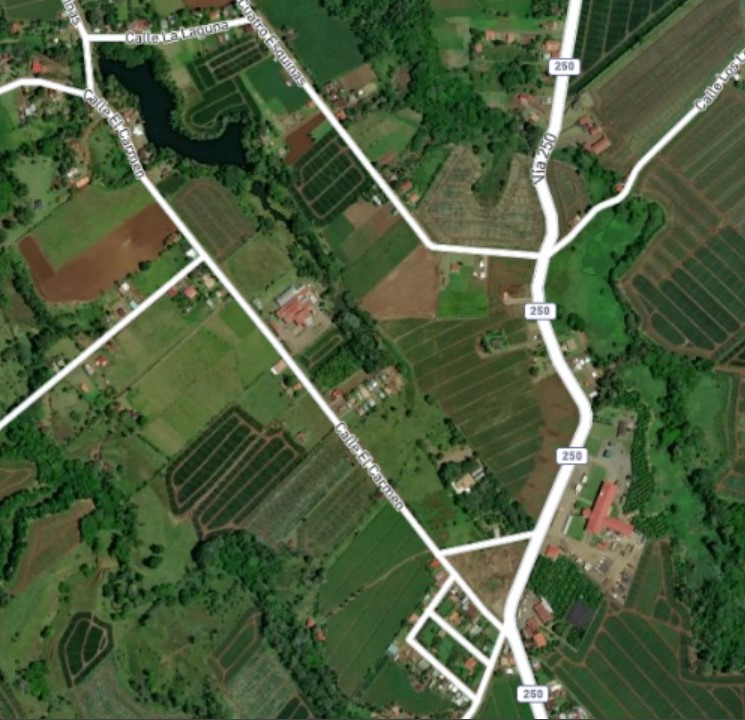
\includegraphics[width=\textwidth]{fig/satelliteZoom.jpg}
\caption{Satellite image corresponding to the polygon surroundings. \textit{Source: terrascope.be}}    
\end{subfigure}
\end{figure}


\begin{figure}[!ht]
\caption[PAL fields centroids and nearest nodes]{PAL fields centroids and nearest nodes. Centroids are coloured blue, and their nearest nodes are coloured red.}  
\label{allNodesPAL}
\centering
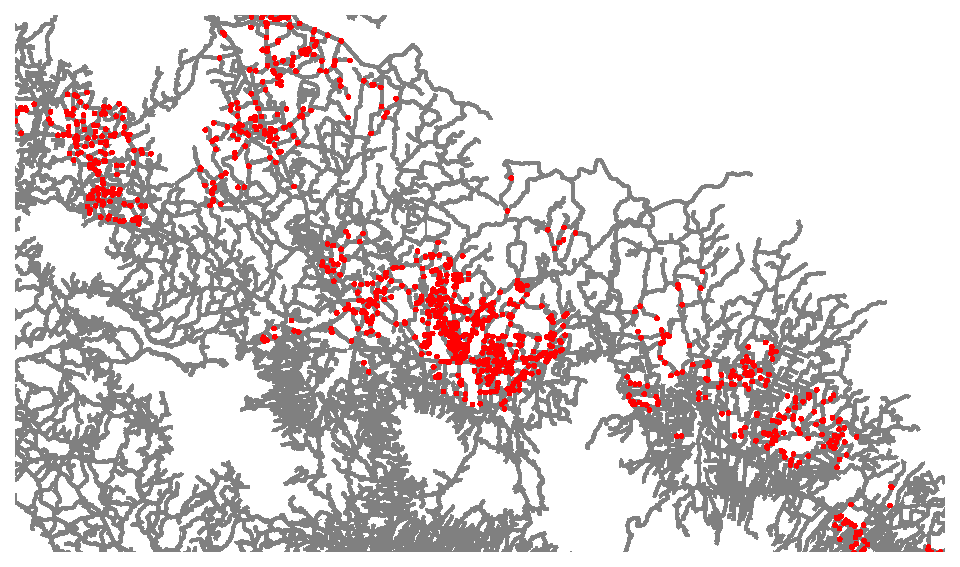
\includegraphics[width = \textwidth]{fig/allNodesNet.pdf}
\end{figure}


\subsection{Processing costs}
\label{costsch4}
The capacity of the facilities, $q_i$, and the costs of setting up a new facility, $f_i$, are estimated using the following data. As mentioned above, we estimate a supply of 4,836,731.25 tonnes of biomass (PAL) per year. Agricultural biogas plants usually have between 100 and 300 kW of power capacity, while industrial units exceed 1,000 kW. For the optimisation, we estimate costs based on 1,000 kW (1 MW) plants due to the important role economies of scale can play \citep{walla2008optimal, pinas2019economic}. Working at full capacity and with a power factor of 0.8, a 1 MW plant can generate 8,760 MWh per year $(0.8 \cdot 1 \si{\MW} \cdot 24 \si{\hour} \cdot 365 \si{\day})$. Assuming that each \si{\meter\cubed} of biogas generates approximately 2 kWh of useable electricity \citep{uddin2016biogas,suhartini2019estimation,swedishBio}, each plant must produce 4,380,000 \si{\meter\cubed} of biogas per year. With a conversion of 25.7 \si{\meter\cubed} per tonne of PAL \citep{arce2014determinacion}, each facility would require 170,428 tonnes (1050 hectares) of PAL each year, or 467 tonnes (3 hectares) every day. 

Capital and operating costs for a biogas plant depend on many factors, and empirical data are not available for the type of plant described in this study. Therefore, for the type of process described above, we provide an estimated range based on an extrapolation from a 250 kW, 137 \si{\tonne \per \day} biogas plant built in 2012 in Costa Rica \citep{sigmaanalysis}, average costs provided by the \citeauthor{ieaBio} and other sources \citep{salerno2017costs, obileke2022economic, newsGuatemala, newsSalvador, ICEbiogas, walla2008optimal}. We estimate that the economic lifespan of each biogas plant is 15 years, the capital costs to be between \$2 and \$4 million, and the annual operating costs to be between \$250 and \$450 thousand. \cref{biogasEstimates} depicts a summary of these estimates. 


\begin{table}[H]
\centering
\begin{threeparttable}
\caption{Estimates for the biogas plant in the optimisation}
\label{biogasEstimates}
\begin{tabular}{ll} 
\hline \hline  
Generator capacity          & 1 MW                      \\
Electricity generation      & 8,760 MWh/yr            \\
Biogas production           & 4,380,000 \si{\meter\cubed}/yr           \\
PAL processed               & 170,428 t/yr           \\
Capital costs               & \$2 to \$4 MM          \\
Operating costs             & \$250 to \$450 M/yr  \\
Facility lifespan           & 15 years                 \\ 
\hline   \hline     
\end{tabular}
\end{threeparttable}%
\end{table}


When deciding the available and suitable locations to place candidate facilities, the criteria present in the literature are varied and, on some occasions, arbitrarily defined. For example, \cite{jeong2019biodiesel}, who developed a supply chain optimisation model for camelina oil-derived biodiesel, selected county centroids as supply sites and also as candidate sites for the construction of new plants. \cite{caballero2007solving} selected candidate facility locations for residual processing plants based, for example, on unemployment rates and the centrality of the towns within the region. \cite{delivand2015optimal} implement well-defined criteria to select candidate facilities that consider planning rules, facility accessibility, and feedstock availability. We find the planning rules particularly relevant and useful when determining candidate facility locations.

Planning rules, also called zoning, are detailed rules on how a certain plot of land or area can be used. A famous example of zoning resolution is that of New York, adopted in 1916 to resolve the issue of property disputes about the height and size of buildings in business areas \citep{weiss1992skyscraper}. In Costa Rica, the zoning regulations are managed by the cantons \citep{planesRegCR}. According to the \citeauthor{PlanesReguladoresPortal}, 40 of the 82 cantons in the country have implemented a zoning regulation. However, most cantons do not publish spatial zoning maps showing which plots of land correspond to the different land uses, and only an official journal establishing the zoning regulations is publicly available. To our knowledge, only the San Carlos canton has developed a map of the zoning plan for the city of Quesada, as shown in \cref{sanCarlosPlan}.

\begin{figure}[!ht]
\caption[Zoning regulation applicable to the city of Quesada]{Zoning regulation applicable to the city of Quesada. Industrial zones are coloured green. \textit{Source: \citep{sancarlosPlan}}}  
\label{sanCarlosPlan}
\centering
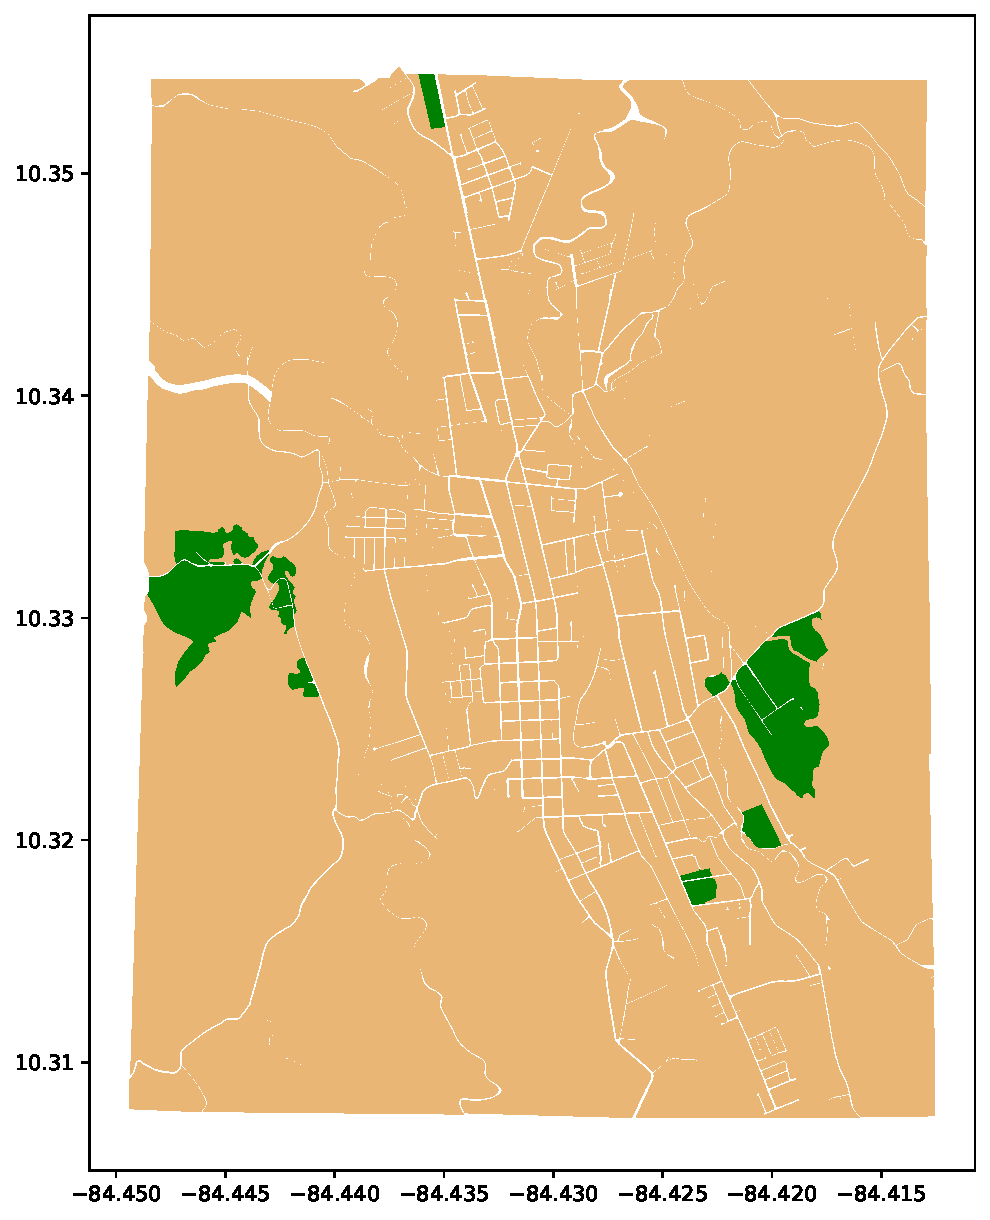
\includegraphics[width = 0.5\textwidth]{fig/sanCarlosPlan.pdf}
\end{figure}

In the case of the city of Quesada, defining potential processing facilities would be straightforward, as these are restricted to industrial zones. Since this type of data is not available for the rest of the country, it is not possible to implement criteria defined by zoning regulations in our FLP. Nevertheless, optimal locations determined by the algorithm can be used as a reference to locate the nearest available and suitable plots of land on a case-by-case basis. Following \citeauthor{delivand2015optimal}, we can at least restrict candidates to accessible locations using the country's road network to choose locations that are accessible by road and that do not fall within protected areas. Therefore, we generated 500 random candidate locations distributed along the street network inside the bounding box of the study area. The method of using network nodes as candidate facilities has been implemented before (e.g., see \cite{zhao2015does}). The generation of random nodes in the network, rather than generating an evenly spaced grid in (decimal) degrees, accounts for the geometry of the graph and guarantees uniform randomness \cite{boeing2017osmnx}. The candidates selected for the optimisation are shown in \cref{candidatesNet}. 

\begin{figure}[H]
\caption{Facility candidates randomly generated over the street network.}  
\label{candidatesNet}
\centering
\includegraphics[width=12cm]{fig/candidatesNet.pdf}
\end{figure}


\subsection{Transportation costs}

As with biogas plants, costs of transportation depend on many factors, and there are no easily accessible data. We estimate, based on several grey literature \citep{van2020cost, transportCost1, transportCost2}, a cost between \$0.20 and \$0.35 tonne-kilometre. We can also make an estimate by calculating the fuel price per kilometre. The fuel consumption of a typical Class 5, medium duty truck used to transport produce in Costa Rica (e.g., Isuzu N-Series with a load capacity of 7-9 tonnes), which is the range of 25-30 \si{l/100~km}. The price of fuel is currently \Colon750 (\$ 1.40) \si{\per \L} \citep{PreciosHistricosRECOPE}. This translates to a fuel cost of \$0.35 \si{\per \km}. This cost does not include any of the other transport-associated costs, such as fixed (e.g., investment costs, insurance) and variable costs (e.g., maintenance), staff costs, and operating costs. Thus, we believe that the estimate of \$0.20 - \$0.35 tonne-kilometre to be plausible. Finally, we should note that we do not consider chargeable weight (1 \si{\meter \cubed} = 333 \si{\kilogram} for road transport) a problem since the proposed solution implies shredding the PAL at the farm, which reduces the volume to a manageable level. The transport costs, $c_{ij}$, are then determined by: 

\begin{equation}
    c_{ij} = p_{tkm} \cdot \sum_{\substack{{i \in U} \\ j \in V}} k_{ij} \ d_j
\end{equation},

where $p_{tkm}$ is the cost per tonne-kilometre and $k_{ij}$ is the distance from the farm $j$ to the facility $i$.

Although it is common in location problems to use the Euclidean distance to calculate distances, the difference between using the road distance and the Euclidean distance is high in some cases \citep{pittayarugsarit2019comparison}. For this reason, we decided to calculate road distances by using the edges of the road network. 

\section{Results}

For the baseline results, we set the facility set-up costs to 3 MM (for a 15 years plant) and the annual operating costs to 350 M. Transportation costs were set at 0.275 tkm. The results obtained from the model consist of the number (30) and locations of biogas plant facilities, and the flows of biomass (PAL) supply from pineapple fields to the facilities. The total cost of the optimal solution is \$30,083,928, from which 16.5 MM are attributed to biogas facilities and 13,6 MM are attributed to transportation. This solution implies processing all the biomass (PAL), 4.9 MM tonnes, produced in the country each year. A map showing the optimal facilities location distribution is depicted in \cref{solutionMAP}. Due to the uncertainty of costs of both facilities and transportation, we analyse the effects of changes in set-up costs and transportation costs and show the different scenarios in the following section. The exact location and the set of facility-field combinations are provided in a CSV file. The MIP model was programmed in Python and solved using the Gurobi Optimiser version 10.0.1. More details can be found in \cref{suplmaterial}. 

\begin{figure}[!ht]
\caption[Spatial representation of the optimal solution for the FLP]{Spatial representation of the optimal solution for the FLP of biogas plants in Costa Rica}
\label{solutionMAP}
\centering
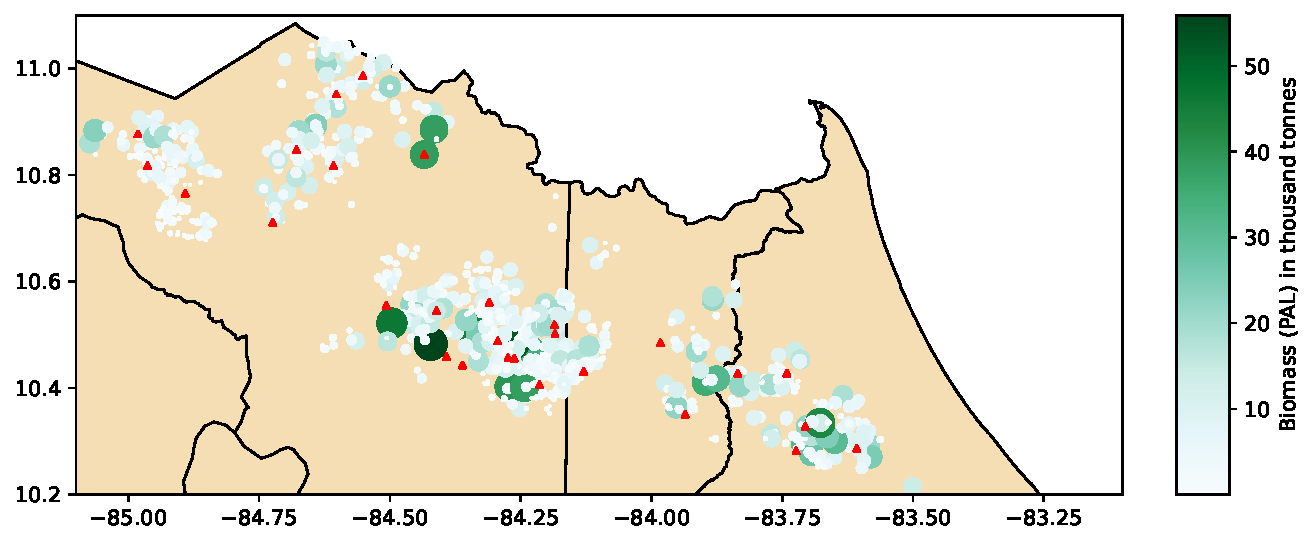
\includegraphics[width=\textwidth]{fig/resultsALL.pdf}
\end{figure}


\subsection{Sensitivity analysis}

We analyse the effect of different cost scenarios on the optimal number of locations. Since the facilities have a maximum capacity, there is a minimum number required to accommodate the entire supply of PAL. As can be seen in \cref{scenarioFLP}, the number of facilities varies depending on the different costs associated with transportation and facility setup. In scenarios with high transportation costs and small facility set-up costs, more facilities are open to minimise distances and costs of transportation. The number of facilities ranges between 28 and 34 and the total cost is between 24.5 and 38.3 MM. 

\begin{table}[H]
\centering
\begin{threeparttable}
\caption[Scenarios for the FLP problem]{Scenarios for the FLP problem. Total annual costs (MM) \& Number of Facilities in parentheses.}
\label{scenarioFLP}
\begin{tabular}{ccccc} 
\hline \hline  
&   & \multicolumn{3}{l}{Transport costs (tkm)} \\
%
&   & 0.20            & 0.275        & 0.35       \\
\multirow{3}{*}{\begin{tabular}[c]{@{}c@{}}Facility set-up\\ costs in \$ MM\end{tabular}}  
& 2 &  (24.5; 28)   &   (28.3; 30)  &  (34.9; 34)  \\
 & 3 & (26.2; 28)   &   (30.1; 30)  &  (36.5; 28)  \\
 & 4 & (28.0; 28)   &   (31.9; 28)  &  (38.3; 28)   \\
\hline   \hline     
\end{tabular}
\end{threeparttable}%
\end{table}


\section{Discussion}

Once the capacity of the plants has been decided, it is trivial to determine the minimum number of facilities needed to process the available PAL in Costa Rica. More interesting is to see how distances and, consequently, the costs of transportation affect the optimal number of facilities in the optimum. In this sense, the location of the supply points is the most important factor in our capacitated FLP problem. In the scenarios with more, less-supplied facilities, the total cost is probably overestimated because the set-up costs are considered for a 1 MW facility, which in such scenarios would not be needed. Nevertheless, the difference should be relatively small considering the small range in the number of opened facilities and the economies of scale attributed to their construction.

The total costs of the FLP, although based on estimates, provide us with a useful visualisation of the benefits an applied solution might bring. If we consider that the total cost to manage the stubble in the field (at least \$1000 per hectare \cite{hernandez2018impacto}) is similar to the average cost shown in \cref{scenarioFLP}, the valorisation of PAL through biogas production does not imply a larger investment in the long term. Additionally, if we consider that the 250,000 MWh of electricity generated from the facilities provide revenues of around \$30 MM (electricity is currently sold at \$0.12 \Colon66.37) per kWh \cite{icePrices2023}) and that the extraction of PAL from the fields allows for faster pineapple production cycles, the valorisation scenario becomes economically reasonable and attractive. Finally, environmental costs should be considered. 

The simplicity of our model allows for new data to be incorporated easily and we expect the model to help in the decision-making process should facilities be built. In this sense, it is relevant to note that, by designing the type of solution described here, we idealise a collective and total solution which takes care of all the supply of PAL in Costa Rica. If pineapple producers were to implement this arrangement, partnerships would be needed to find a cost-effective solution. Considering that cooperatives are common in the pineapple industry, we consider this arrangement plausible. Another scenario we consider is that of an external company setting up a supply chain to collect, transport, and process the PAL. In such a case, an arrangement similar to that of municipal solid waste can be considered, with benefits for both pineapple producers and biogas producers.

The FLP has many variants, allowing for the modelling of different situations with different objective functions and constraints. The simple model shown here provides a solution for a tailored capacitated, multi-facility problem. Ideally, the model would optimise not only the number and location of a given type of capacitated facility but also the optimal capacity of the facilities accounting for economies of scale, i.e., for the different costs associated with processing one extra tonne of PAL in a facility with given fixed and variable costs. Two examples of this type of FLP can be found in \cite{wetterlund2012optimal, nordin2022optimal}. This type of FLP can provide more precise solutions which might involve building facilities of different sizes throughout the network, and its implementation is recommended.

\subsection{Extension of the model}

Cost minimisation is at the core of any operational challenge a company might face. FLP is a useful tool for stakeholders to consider options before making large, long-term investments. As exemplified in \cref{FLPlit}, FLP has expanded to incorporate environmental costs. When there is more than one objective to minimise, the FLP becomes a multi-objective MIP, which increases the complexity of the optimisation. The formulation of an environmental costs minimisation function is analogous to the economic costs minimisation function:

\begin{equation}
\label{envObjFun}
    \text{Min} \sum_{i \in U} \sum_{j \in V} e\_t_{ij} \ e\_f_{ij} + \sum _i \ y_i,
\end{equation} 

subject to the same constraints as \cref{objectivefun}, and where $e\_t_{ij}$ are the environmental impacts (usually measured in $CO_2$ emissions emitted) from transport between farm $j$ and the facility $i$, and $e\_f_{ij}$ are the environmental impacts associated with setting up and operating facility $i$. Similar to the operational costs function, the objective is to find the best number and location of facilities that minimise the total environmental impact of transportation and facilities. The complexity of the problem arises due to the nature of multi-objective MIPs, where the solution is expressed as a set of Pareto optima that represent the optimal trade-offs between the minimisation objectives. Since no single solution can be found, the challenge is to identify the preferable Pareto solution from the set based on given criteria and analysis of decision-makers \cite{limleamthong2018combined}. Usually, the Pareto frontier is shaped such that a solution with relatively low environmental impact can be chosen before the curve steepens towards relatively high economic costs. At that point, the gains from taking more environmentally friendly solutions are small compared to the very high economic costs \cite{harris2009multi}.

Biogas production, especially with second-generation feedstock such as PAL, has environmental benefits in terms of global warming potential and resource consumption compared to energy supply from fossil fuels. Furthermore, the environmental impacts of the construction and demolition of a biogas plant are relatively small, especially if a high utilisation ratio (long service life) of the plant is achieved \cite{hijazi2016review}. Thus, since the emissions from transportation can become significantly large, we expect the inclusion of environmental costs in the analysis to produce scenarios with a greater number of less-capacitated facilities. It is recommended to explore and implement a multi-objective FLP that accounts for both operational and environmental costs if a truly sustainable solution is to be obtained. 

\section{Conclusion}

The third set of research questions laid out in \cref{researchQ} has been answered throughout this chapter. The suitable locations and optimal spatial distribution of PAL processing plants were identified using the FLP making some simplifying assumptions about a potential real-case scenario. Deciding whether the processing of PAL should be centralised or decentralised depends on the type of valorisation process that is implemented. In the case of biogas production, a decentralised solution is more suitable for the case of Costa Rica considering the spatial distribution of pineapple fields in the country and the biomass processing capacity of biogas plants. The average scenario implies the construction of 30 biogas plants with a total annual cost of \$30.1 MM. Moreover, the results inform how the implementation of a biogas production scenario can provide operational cost savings to the pineapple industry in Costa Rica. 

Taking into account the uncertainty surrounding possible PAL valorisation solutions in Costa Rica, this study provides an optimistic initial step toward the implementation of a large-scale valorisation process. Should different types of valorisation techniques be considered, either as an alternative or an addition, this model provides the tools to analyse the most cost-effective operational solution. Since several value-added goods can be produced with PAL, as described in \cref{neweconomy}, we contemplate the addition of other processes to the biogas production chain, e.g., fibre extraction from the leaves prior to anaerobic digestion. This cascading solution would take advantage of the supply chain to integrate processes and generate greater value. From the FLP design point of view, this might require modelling a multi-echelon problem which would account for the distribution of PAL-based products to demand points. 

The analysis produced here is limited by the available data and, thus, stringent assumptions and simplifications were made. As more data on the potential costs, capacity, and production of PAL-fed biogas plants are known, more accurate results from the model will be obtained. Furthermore, the potential locations of the facility used in the analysis were randomly selected from the network nodes. This ensures connectivity in the network but does not consider regulations related to zoning or land availability. A true solution will be close to the one provided in the study, but these considerations must be taken into account. Finally, we recognise the importance of accounting for environmental impacts when finding FLP solutions, as these might change the number and spatial arrangement of facilities considerably. Estimating such impacts can also shed light on the environmental costs of valorising PAL compared to managing it in the field with agrochemicals and burning. Since PAL is a second-generation feedstock and does not compete with other crops or land use, we expect the costs to be relatively low.

\newpage\cleardoublepage
\chapter{Conclusion and Reflection}
\label{concludeGen}

\section{Summary of the main findings of the study}

1. Summarise the main contributions and findings of the study. I would divide this part in three:

2. Explanation of how the FCM helps us understand the current situation, and what the experts in the industry expect. 

3. What the FLP tells us about the location of processing plants and the possibilities to process PAL in CR. 

4. Explain the stage of development of the valorisation options, what seems to be the best way (probably a mix of many options chained to each other). Also sum up the difficulties to valorise and what is being done at the moment. 

\section{Implications of the results for the valorisation of pineapple stubble}

1. Discuss the implications of the research for practice and policy. 

2. The FCM is relevant to understand the challenges and to know what's needed from a policy point of view. How can stakeholders be incentivised. This will eventually speed up the valorisation systematically.

3. How the FLP, and in general spatial optimisation, is key to reduce costs and incentivise stakeholders to start valorising in mass. The results can reduce uncertainty. 

4. Explain how there's still a lot of improvement to be made in the technology of the pineapple valorisation options. There is technology, but most is not tailored to the PAL valorisation, and a lot of trial and error is still needed to have an out-of-the-box solution that can be applied at a large scale. 

\section{Recommendations for future research and practical applications}

2. First, recommendations on specific aspects of the system that need more attention. If it turns out that collaboration in the system is crucial (from the FCM), then researches can continue analysing how to improve this, and stakeholders should put effort in making bridges. 

3. Depending on the results from the spatial optimisation, it would be a good idea to delve deeper in this study, or to analyse more factors related to the logistics of the valorisation. 

4. Since the valorisation process is in its early stages, the creation of knowledge, the collection of data, and the spread of these two, is paramount to reach new stepping stones. For example, a MCDA, or a LCA will be valuable, but data is not present at the moment. Then we can make a comparative study of the economic feasibility of the options.

5. For stakeholders, I think it's relevant pointing out the importance of small steps. This is a process that takes time, and the system in which the valorisation unfolds is complex. Stakeholders should be incentivised to try ways to valorise, even if it's to a small extent. If everyone tries something and shares their results, more knowledge can be gathered for faster advancements.

\section{Reflection about the study}

1. If possible, I would like to give my reflection of the study, in terms of my thinking evolution throughout the thesis development.

2. First, a reflection on field work and qualitative analysis from the point of view of an economist and how challenging it can be. How qualitative analysis can be both useful and tricky to use. And what can be learnt from people in the ground as opposed to literature review/numbers. Systems are more complex than I thought, and it's important to keep this in mind when using models or doing quantitative analysis.

3. A comment on center-periphery structure, and on consumption in developed countries and the globalisation of food production. It is important to understand that the environmental problems of the stubble in CR exist because of the global dynamic of consumption and the historical dynamic of centre and periphery. Developing countries have the challenge to become sustainable in an era of climate crisis, when developed countries can presume of becoming green at a lower social cost.

\newpage\cleardoublepage

\bibliographystyle{apalike}

\chapter*{Bibliography}
\addcontentsline{toc}{chapter}{Bibliography}
\bibliography{bib/MScThesis.bib}

\chapter{Appendix}

\renewcommand{\thesection}{A\arabic{section}}
\renewcommand\thefigure{A\arabic{section}.\arabic{figure}}  
\renewcommand\thetable{A\arabic{section}.\arabic{table}}  

\section{FCM results}

\subsection{Experts and Stakeholders Interview Outline}
\label{interviewOutline}

\begin{itemize}

\item Name, organisation, the purpose of the organisation.
\item What do you understand by Circular Economy?
\item What do you understand by \textit{valorisation of stubble}?
\item What is the current situation of the valorisation of stubble in Costa Rica?
\item What factors influence the valorisation of Costa Rican pineapple stubble? Please indicate at least four. \textit{(Sector structure)}
\item What factors are influenced by the valorisation of Costa Rican pineapple stubble? \textit{(Outcome)}
\item Is there a relationship between the factors described? How would you describe those relationships? Positive, neutral, or negative?
\item Identify three key drivers that can boost the valorisation of pineapple stubble and, consequently, the circularity of the Costa Rican pineapple sector. Think of the national, international scale, factors external to the production chain.
\item Do you perceive any trends in the factors previously mentioned in the last 5 years?
\item Who are the most important actors in the stubble valorisation process?
\item Which valorisation options seem most feasible to you, and why? Think about the technological, economic, and commercial aspects of valorisation.

\end{itemize}



\subsection{Concepts Description}
\label{conceptsGlossary}

\begin{xltabular}{\textwidth}{XX}
\caption{Concepts present in the FCM and their description}
\label{conceptsList} \\

 \hline \hline  \multicolumn{1}{|c|}{\textbf{Concept}} & \multicolumn{1}{c|}{\textbf{Description}} \\ \hline 
\endfirsthead

\multicolumn{2}{c}%
{\tablename\ \thetable{} -- continued from previous page} \\
 \hline \hline  \multicolumn{1}{|c|}{\textbf{Concept}} & \multicolumn{1}{c|}{\textbf{Description}} \\ \hline 
\endhead

\hline \multicolumn{2}{|r|}{{Continued on next page}} \\ \hline
\endfoot

\hline
\endlastfoot


Regulation of stubble management &
  Regulate how the stubble can be managed (what agrochemicals can be used,  when is fire allowed, etc.). \\ \hline
Good image of the industry &
  How consumers, investors, the government, and the population perceive the industry. \\ \hline
Collaboration/Communication &
  Between pineapple companies, academia, government, social communities, and other industries. \\ \hline
Pollution (soil, air and water) &
  Refers to the presence of substances or particles in amounts that can be harmful to human health and ecosystems. \\ \hline
Cost of fossil fuel-based materials &
  Cost of materials used in the industry that come directly or indirectly from fossil fuels (plastics, agrochemicals, and other materials). \\ \hline
Customs of the industry &
  Practices that have been present for many years and inherited by new generations of pineapple producers. \\ \hline
Demand of PAL products &
  Demand for products derived, completely or partially, from PAL (e.g., biobased materials to replace plastics, bioenergy and biofuels, textiles). \\ \hline
Uneven terrain &
  In the pineapple plantations. In a broader sense, it refers to the inaccessibility of the terrain. \\ \hline
Land availability &
  Availability of the land to plant. As long as there is stubble in the field, the land is not available. \\ \hline
Employment &
  The number of people employed in the PA industry or in a PAL-related industry. \\ \hline
Extraction from the field &
  Extracting the PAL from the field. \\ \hline
Funding &
  Public or private funding, either national or international. \\ \hline
International instability &
  Lack of stability or predictability in the international system. It can be political instability, economic uncertainty, or military conflicts. \\ \hline
Innovation &
  Innovation related to the valorisation of PAL. Creation of new ideas, products, or methods. \\ \hline
Research &
  Carried out by universities and other scientific centres. \\ \hline
Rain &
  Precipitation in the terrain and the road network inside and outside the field. \\ \hline
Stable fly &
  Number of stable flies. \\ \hline
Government presence &
  How involved are local and national governments in the pineapple sector and PAL-valorisation development. \\ \hline
Green consumers &
  Consumers who demand products that have undergone an eco-friendly production process and that safeguards the planets' resources. \\ \hline
Pineapple production productivity &
  Amount or weight of fruit produced per unit of land, labour, or other resources used. \\ \hline
Labour productivity &
  The efficiency with which labour is used in the production of goods. Total value of production / Total number of hours worked. \\ \hline
Import regulations and standards &
  That other countries impose to exporters from CR. \\ \hline
Profitability of pineapple companies &
  Company's ability to generate profit. \\ \hline
Business risk &
  All events that may affect or cause losses to a company within the framework of its economic activity. \\ \hline
Community's health/well-being &
  Health and social and environmental well-being of the communities directly or indirectly affected by PA production. \\ \hline
Industry sustainability &
  Practice of using natural resources in a way that preserves them for future generations. \\ \hline
Company  size &
  Refers to the amount of resources that the company has: hectares, workers, machinery. \\ \hline
Industry's transparency/openness &
  Regarding operations, cultivation methods, use of supplies and stubble management. \\ \hline
Use of agrochemicals &
  Chemicals used in to enhance crop growth, protect against pests and diseases, and manage the stubble (fertilizers, herbicides, insecticides). \\ \hline
valorisation of PAL &
  Activities that convert PAL into new products or materials. \\ \hline
Soil fertility &
  Ability of the soil to support plant growth. \\ \hline
Ranchers' productivity &
  It can be measured in terms of the number of animals raised, the amount of meat or milk produced, the value of their sales, or the profits they generate.

\end{xltabular}

\clearpage


\subsection{FCM Quantitative Aggregation}
\label{quantitativeAgg}

For the quantitative aggregation, the FCMpy package, a Python package for building FCMs and implementing scenario analysis, was used \citep{mkhitaryan2022fcmpy}. The data extracted from the questionnaire responses were transformed to fit the structure required to use the package. We aggregate the responses by converting the categorical ratings to numerical weights. Sometimes, researchers use a scale to weigh the consistency of stakeholders' answers, giving more weight to experts who are believed to be more knowledgeable. In our case, we have assumed that all individual FCMs are equally valid and, thus, the same weight was applied to all maps. Aggregation of individual FCMs can be performed in several ways, the averaging of all individual matrices being the simplest \citep{jetter2014fuzzy}. This aggregation approach is usually followed by normalisation of the values to narrow the weights of the connections in the range [-1, 1]. Several examples using this approach can be found in the literature (see \citep{lopolito2020combined, morone2021using, morone2019promote}. In other cases, the authors do not explicitly explain the method used, and it is simply mentioned that the aggregation is handled by the software selected to perform the analysis \cite{konti2022determinants, kokkinos2020circular, falcone2020use}. In our case, we implement fuzzy logic to perform the aggregation of individual FCMs, as recommended by the developers of the FCMpy package. The aggregation via fuzzy logic, although not common, has been used in the past \citep{nasirzadeh2020modelling, amini2022combined}. This method has the advantage of using membership function maps, which are useful when it is hard to define a specific cutoff value for a linguistic term \citep{wang2015study}. Thus, this technique is well-suited to FCM applications where the input is created from human expert knowledge. 

Conversion to numerical weights requires four steps: 1) define the fuzzy membership functions, 2) apply a fuzzy implication rule, 3) combine the membership functions, and 4) defuzzify the aggregated membership functions to derive numerical causal weights \citep{mkhitaryan2022fcmpy}. In Step 1) we define a triangular membership function that represents the linguistic terms, as can be observed in \cref{trapmf}. Step 2) requires calculating the proportion of the answers to each linguistic term for a given concept and then applying a fuzzy implication rule to allocate the weights to the corresponding membership functions. The Mamdani minimum fuzzy implication rule is used, which applies a function to compute the element-wise minimum of the array elements to cut the membership function at the endorsement level, as shown in \cref{mamdani}. The aggregation of the membership function takes place in step 3), using a fMax function, simply computing the element-wise maximum of array elements, in this case, to ``merge" the membership functions, resulting in a single shape representing the level of endorsement for a particular connection. Finally, we defuzzify the aggregated functions using the centre-of-gravity method, resulting in a single value for each concept, as shown in \cref{defuzz}. At the end of the aggregation of individual FCMs via fuzzy logic, we obtain a value for each connection representing its social (aggregated) weight. In practice, the result is a matrix $n \times n$ whose element $ E_{ij} $ indicates the value of the weight $ W_{ji} $ between concept $ C_{j} $ and concept $ C_{i} $. 



\begin{figure}\centering
\subfloat[Triangular membership functions]{\label{trapmf}\includesvg[width=.45\linewidth]{fig/trapmf.svg}}\hfill
\subfloat[Fuzzy implication rules]{\label{mamdani}\includesvg[width=.45\linewidth]{fig/mamdani.svg}}\par 
\subfloat[Defuzzification of the aggregated membership functions]{\label{defuzz}\includesvg[width=.45\linewidth]{fig/defuzz.svg}}
\caption*{Adapted from \cite{mkhitaryan2022fcmpy}}
\label{FCMpy}
\end{figure}


With the aggregated matrix, we can now perform a dynamic analysis of the FCM. As \cite{edwards2021building} mention, in a mathematical sense, the output of the analysis is static rather than dynamic, so they adopt the term ‘quasi-dynamic’ to indicate the dynamic character of the interpretation of the changes in the system. This quasi-dynamic analysis allows us to see where the system will go if things continue as they are, i.e., to determine the steady state of the system \citep{ozesmi2004ecological}. The steady-state value taken by each concept reflects its importance within the system according to stakeholders' knowledge and provides an idea of the evolution of the system in current circumstances \citep{lopolito2020combined}. 

To compute the steady state of the system, a vector of initial states of variables (usually set to 0 or 1) is first multiplied by the aggregated adjacency matrix of the FCM. Then, the resulting transformed vector is repeatedly multiplied by the adjacency matrix and transformed until the system converges to a steady state. To maintain the values in the range [0,1] and reach a steady state, an inference method, including a threshold function, is used in each iteration:

\begin{equation}
\label{equation1} 
A_i^{t+1} = f \left( A_i + \sum_{j=1}^{n} A_j^t W_{ji} \right), 
\end{equation}

where $A_i^{t+1}$ is the value of concept $C_i$ in the simulation step $t+1$, $A_i^{t}$ is the value of concept $C_i$ at simulation step t, $A_j^{t+1}$ is the value of concept $C_j$ at time t, $W_{ji}$ is the weight of the interconnection from concept $C_j$ to concept $C_i$, and $f$ is the Sigmoid bounded monotonic increasing function in the form

\begin{equation}
\label{equation2}  
f(x) = \frac{1}{1+e^{-\delta x}}, \quad  x \in \mathbb{R}, 
\end{equation}

where $x$ is the defuzzified value and $\delta$ is a steepness parameter for the Sigmoid function. Note that this non-negative transformation allows a better understanding and representation of activation levels of variables \citep{ozesmi2004ecological}. The inference method shown in \cref{equation1} is the modified Kosko function, a modified version of the Kosko rule that is suitable when we require updating the activation value of concepts that are not influenced by other concepts \citep{sujamol2018study}. A rescaled inference rule is also included in most FCM packages and software programmes, although its properties are not well explained. To our knowledge, the rescaled inference rule was introduced by \cite{papageorgiou2011new} to avoid conflicts in which the initial values of the concepts are 0 or 0.5, or in cases where the initial values of concepts are not known. However, this inference method was applied in the context of health informatics, and therefore we decided not to consider it for our study. 

It is important to note that iterations are not related to time. This property allows an interpretation of the dynamics of the different factors relative to the other factors or relative to other descriptions of the system \citep{edwards2021building, diniz2015mapping}. In this sense, it is possible to evaluate different scenarios and outcomes by asking ``what-if" questions and simulating different conditions or policy choices. This can be used to compare what policy decisions or changes in the system would have the greatest effect on the variables of interest.



\clearpage

\subsection{Entropy results}
\label{entropyResults}

\begin{xltabular}{\textwidth}{XXc}
\caption{Entropy values of FCM connections}
\label{entropyFCM} \\

\hhline{===}\multicolumn{1}{|c|}{\textbf{From concept}} & \multicolumn{1}{c|}{\textbf{To concept}} & \multicolumn{1}{c|}{\textbf{Entropy}}\\ \hline 
\endfirsthead

\multicolumn{3}{c}%
{\tablename\ \thetable{} -- continued from previous page} \\
\hhline{===}  \multicolumn{1}{|c|}{\textbf{From concept}} & \multicolumn{1}{c|}{\textbf{To concept}} & \multicolumn{1}{c|}{\textbf{Entropy}}\\ \hline 
\endhead

\hline \multicolumn{3}{|r|}{{Continued on next page}} \\ \hline
\endfoot

\hhline{===}
\endlastfoot

IndustryTransparency & collabComms & 1.750000 \\
academia & innovation & 1.905639 \\
agrochemicalsUse & pollution & 1.405639 \\
businessRisk & innovation & 2.155639 \\
collabComms & innovation & 0.954434 \\
communityHealth & industryImage & 1.298795 \\
\multirow[c]{2}{*}{companySize} & funding & 1.905639 \\
 & pineappleProdProfitability & 1.905639 \\
\multirow[c]{2}{*}{costFFmaterials} & palProductsDemand & 2.155639 \\
 & pineappleProdProfitability & 1.905639 \\
\multirow[c]{2}{*}{employment} & communityHealth & 1.405639 \\
 & funding & 2.155639 \\
\multirow[c]{3}{*}{fieldExtraction} & agrochemicalsUse & 1.500000 \\
 & innovation & 2.155639 \\
 & palvalorisation & 2.155639 \\
\multirow[c]{2}{*}{funding} & academia & 1.405639 \\
 & innovation & 1.811278 \\
\multirow[c]{2}{*}{govtPresence} & collabComms & 1.750000 \\
 & stubbleMgmtRegulation & 1.750000 \\
\multirow[c]{2}{*}{greenConsumers} & agrochemicalsUse & 2.155639 \\
 & palProductsDemand & 1.905639 \\
importRegulations & agrochemicalsUse & 1.561278 \\
industryCustoms & palvalorisation & 2.405639 \\
industryImage & funding & 2.155639 \\
industrySustainability & palProductsDemand & 1.905639 \\
\multirow[c]{3}{*}{innovation} & fieldExtraction & 1.298795 \\
 & laborProductivity & 1.905639 \\
 & palvalorisation & 1.561278 \\
intInstability & costFFmaterials & 1.561278 \\
laborProductivity & fieldExtraction & 2.500000 \\
landAvailable & pineappleProdProductivity & 2.155639 \\ \\
\multirow[c]{2}{*}{palProductsDemand} & innovation & 1.561278 \\
 & palvalorisation & 1.500000 \\
\multirow[c]{7}{*}{palvalorisation} & agrochemicalsUse & 2.155639 \\
 & fieldExtraction & 1.405639 \\
 & industrySustainability & 1.500000 \\
 & landAvailable & 1.561278 \\
 & pineappleProdProfitability & 2.000000 \\
 & soilFertil & 1.561278 \\
 & stableFly & 2.155639 \\
pineappleProdProductivity & pineappleProdProfitability & 1.405639 \\
pineappleProdProfitability & industrySustainability & 1.750000 \\
pollution & communityHealth & 1.061278 \\
rain & fieldExtraction & 2.155639 \\
\multirow[c]{2}{*}{stableFly} & communityHealth & 1.405639 \\
 & ranchersProductivity & 1.750000 \\
\multirow[c]{5}{*}{stubbleMgmtRegulation} & agrochemicalsUse & 2.500000 \\
 & industrySustainability & 1.905639 \\
 & innovation & 1.500000 \\
 & palvalorisation & 1.750000 \\
 & stableFly & 1.750000 \\
unevenTerrain & fieldExtraction & 2.405639 \\
\end{xltabular}



\subsection{FCM matrix}

\begin{figure}[H]
\caption{FCM weight matrix} 
\label{FCMMatrix}
\centering
\makebox[\textwidth][c]{\includesvg[width=\textwidth]{fig/matrixFCM.svg}}%
\end{figure}

\section{Supplementary material}
\label{suplmaterial}

The scripts and data used for the Fuzzy Cognitive Mapping and the Facility Location Problem are publicly available in this \underline{\href{https://github.com/isaldiviagonzatti/MscThesis}{GitHub repository}}. For more information, read the README file in the repository. 
\newpage\cleardoublepage

 
\end{document}